\documentclass[final,5p,times]{elsarticle}
\usepackage{amsmath,amssymb,amsfonts}
\usepackage{amsthm}
\usepackage{graphicx}
\graphicspath{{figs/}}
\usepackage{booktabs}
\usepackage{algorithm}
\usepackage{algorithmic}
\usepackage{textcomp}
\usepackage[hidelinks]{hyperref}
\usepackage{microtype}
\setlength{\emergencystretch}{2em}
\usepackage{placeins}
\usepackage{mathtools}
\usepackage{tikz}
\usetikzlibrary{arrows.meta, positioning, shapes.geometric, fit}
%% Float-placement tuning: allow wide figure* floats to share a page
%% top with text so they are placed as soon as possible.
\setcounter{topnumber}{4}
\setcounter{dbltopnumber}{3}
\setcounter{totalnumber}{8}
\renewcommand{\topfraction}{0.92}
\renewcommand{\dbltopfraction}{0.92}
\renewcommand{\textfraction}{0.07}
\renewcommand{\floatpagefraction}{0.75}
\renewcommand{\dblfloatpagefraction}{0.85}
\theoremstyle{plain}
\newtheorem{theorem}{Theorem}
\newtheorem{lemma}{Lemma}
\newtheorem{proposition}{Proposition}
\newtheorem{corollary}{Corollary}
\theoremstyle{definition}
\newtheorem{assumption}{Assumption}
\newtheorem{definition}{Definition}
\theoremstyle{remark}
\newtheorem{remark}{Remark}
\DeclareMathOperator{\diag}{diag}
\DeclareMathOperator{\col}{col}
\DeclareMathOperator{\row}{row}
\DeclareMathOperator{\rank}{rank}
\DeclareMathOperator{\vecs}{vecs}
\newcommand{\R}{\mathbb{R}}
\newcommand{\C}{\mathbb{C}}
\newcommand{\ones}{\mathbf{1}}
\newcommand{\bx}{\boldsymbol{x}}
\newcommand{\bu}{\boldsymbol{u}}
\journal{IFAC Journal of Systems and Control}
%% Suppress the "Preprint submitted to ..." first-page footer.
\makeatletter
\def\ps@pprintTitle{%
  \let\@oddhead\@empty
  \let\@evenhead\@empty
  \def\@oddfoot{\centerline{\thepage}}%
  \let\@evenfoot\@oddfoot}
\makeatother
\begin{document}
\begin{frontmatter}
\title{Data-Driven Q-Learning for Consensus and Multi-Consensus Control of Discrete-Time Linear Multi-Agent Systems}
\author[ttu]{Md~Nur-A-Adam~Dony}
\ead{mdony42@tntech.edu}
\author[ttu]{Syed~Ali~Asad~Rizvi\corref{cor}}
\ead{srizvi@tntech.edu}
\cortext[cor]{Corresponding author.}
\address[ttu]{Department of Electrical and Computer Engineering, Tennessee Technological University, Cookeville, TN 38505, USA}
\begin{abstract}
This paper presents data-driven Q-learning algorithms for consensus and multi-consensus control of discrete-time linear multi-agent systems. Both state feedback and output feedback formulations learn the gains of a predictor-based consensus protocol directly from measured data, without knowledge of the agent dynamics. The state feedback algorithm recovers both gains from a single agent's state-input trajectory, with convergence to the discrete algebraic Riccati equation solution established rigorously. The output feedback extension learns the input-coupling gain and reconstructs the inter-agent disagreement feedback from input-output data alone, eliminating full state measurement while preserving the consensus properties of the underlying design. Every example is validated under both feedback types, and the state feedback and output feedback deployments are shown to produce trajectories that coincide to machine precision, as the theory predicts. A numerical robustness analysis demonstrates the advantage of the data-driven gains under parametric model uncertainty, and simulations on multi-consensus, formation control, and vehicle-platoon scenarios validate the results against the model-based benchmark.
\end{abstract}
\begin{keyword}
Multi-agent systems \sep Consensus control \sep Q-learning \sep Output feedback \sep Data-driven control \sep Discrete-time systems
\end{keyword}
\end{frontmatter}
%% ===================================================================
\section{Introduction}
\label{sec:intro}
%% ===================================================================
Consensus control of networked multi-agent systems (MAS) is a fundamental problem in distributed control theory, with applications in formation control of unmanned vehicles~\cite{francis2016,dony2021distributed,dong2020tracking}, synchronization of complex networks~\cite{dorfler2014,li2010}, distributed filtering~\cite{battistelli2014}, and opinion dynamics in social networks~\cite{proskurnikov2017}. The central objective is to design distributed control laws that drive all agents toward common trajectories using only local information exchanged over a communication graph.

A well-known challenge distinguishes the discrete-time and continuous-time settings. For continuous-time MAS, arbitrarily fast convergence to consensus can be achieved simply by increasing the scalar coupling gain~\cite{li2014,liu2021}. In sharp contrast, for discrete-time systems, the coupling gain is constrained to be small---typically inversely proportional to the largest eigenvalue of the Laplacian matrix---to maintain closed-loop stability~\cite{ma2015,ren2010,xiao2004}. This constraint fundamentally limits the achievable convergence rate.

Recently, Cacace et al.~\cite{cacace2024} proposed a predictor-based consensus protocol for discrete-time LTI MAS that overcomes this limitation through an implicit feedback law involving both the state and input of neighboring agents, recovering arbitrary convergence rate via multiple consensus steps per sampling period. The analysis extends to weakly connected digraphs through almost equitable partitions~\cite{monaco2019}, and the design requires solving a single discrete algebraic Riccati equation (DARE) for two gain matrices $F$ and $G$. However, this requires exact knowledge of $(A,B)$, which may not be available in practice due to modeling errors, parametric variations, or discretization approximations~\cite{dony2020tracking,dong2020tracking,dony2021robust}.

Reinforcement learning (RL) offers a model-free alternative~\cite{lewis2009}: Q-learning solves the LQR problem without system knowledge~\cite{bradtke1994} via policy iteration (PI) or value iteration (VI), and output feedback RL reconstructs the state from input-output data~\cite{rizvi2022}. For MAS, Zhang et al.~\cite{zhang2011} developed RL-based optimal synchronization; related data-driven methods include safe RL for discrete event systems~\cite{dony2025debf}, battery balancing~\cite{dony2026battery}, and Koopman-based control~\cite{dony2024koopman}. All of these, however, address the standard explicit protocol $u_i = -\kappa \sum_j F(x_i - x_j)$; the protocol of~\cite{cacace2024} is implicit---$u_i$ depends on neighbors' states \emph{and inputs} through $G$---which prevents their direct application. Integrating model-free RL with predictor-based consensus has not been addressed.

\emph{Statement of novelty.}\ In this paper, we learn the consensus gains of the predictor protocol of~\cite{cacace2024} directly from data. The entry point is structural: the consensus DARE coincides with the LQR Riccati equation for $R = I_m$, so single-agent Q-learning can extract both gains $F$ and $G$ without knowledge of $(A,B)$. This equivalence is not itself the contribution; a direct composition of established Q-learning~\cite{bradtke1994,lewis2009,rizvi2022} with the protocol fails on three counts that the paper resolves: (a)~the protocol is implicit in $u_i$ through $G(u_i-u_j)$, which blocks existing RL-based MAS methods~\cite{zhang2011}; (b)~output-feedback Q-learning returns the absolute regulator $-K^*x_i$, which drives each agent to the origin, so consensus instead requires reconstructing the inter-agent disagreement $F(x_i-x_j)$ from input-output data (Proposition~\ref{prop:disagreement}); and (c)~only \emph{exact} recovery of the DARE solution preserves the arbitrary convergence rate of~\cite{cacace2024}. To the best of our knowledge, this is the first work to (i)~decouple the learning of the predictor gains $(F,G)$ from the network topology, so that one agent's data serves any network; (ii)~reconstruct the inter-agent disagreement feedback purely from input-output filter states, with no observer and no identification; (iii)~establish exact inheritance of all consensus and multi-consensus guarantees, including an extension of the stability condition of~\cite{cacace2024} to the positive semi-definite weights $Q = C^\top Q_y C$ that output feedback necessitates (Lemma~\ref{lem:psdQ}); and (iv)~validate every scenario under both feedback types with the two deployments coinciding to machine precision. Table~\ref{tab:comparison} summarizes the distinctions.

\emph{Organization.}\ Section~\ref{sec:methods} sets the preliminaries, recalls the predictor-based protocol, states the problem, and develops the state and output feedback Q-learning algorithms with complete convergence proofs. Section~\ref{sec:results} reports the simulation studies. Section~\ref{sec:discussion} analyzes complexity, scalability, communication, and limitations. Section~\ref{sec:conc} concludes.
\begin{table*}[!t]
\centering
\caption{Comparison of the proposed framework with existing methods.}
\label{tab:comparison}
\small
\setlength{\tabcolsep}{6pt}
\begin{tabular}{lccccc}
\toprule
Feature & Cacace et al.~\cite{cacace2024} & Zhang et al.~\cite{zhang2011} & Bradtke et al.~\cite{bradtke1994} & Rizvi--Lin~\cite{rizvi2022} & \textbf{Proposed} \\
\midrule
Model-free & No & Yes & Yes & Yes & \textbf{Yes} \\
Output feedback & No & No & No & Yes & \textbf{Yes} \\
Arbitrary conv.\ rate & Yes & No & N/A & N/A & \textbf{Yes} \\
Single-agent learning & N/A & No & Yes & Yes & \textbf{Yes} \\
Implicit $G(u_i{-}u_j)$ coupling & Yes & No & No & No & \textbf{Yes} \\
Multi-consensus & Yes & No & No & No & \textbf{Yes} \\
\bottomrule
\end{tabular}
\end{table*}
%% ===================================================================
\section{Methods}
\label{sec:methods}
%% ===================================================================
Section~\ref{subsec:prelim} sets the preliminaries, Section~\ref{subsec:protocol} recalls the predictor-based protocol and its model-based design, Section~\ref{subsec:problem} states the problem, and Sections~\ref{sec:sf_ql}--\ref{sec:ofb_ql} solve it under state and output feedback.
\subsection{Preliminaries}
\label{subsec:prelim}
Consider a digraph $\mathcal{G} = (\mathcal{V}, \mathcal{E})$ with $|\mathcal{V}| = N$ nodes, in-neighbor sets $\mathcal{N}_i = \{j : (j,i) \in \mathcal{E}\}$, in-degrees $d_i = |\mathcal{N}_i|$, and Laplacian $\mathcal{L} = \mathcal{D} - \mathcal{A}$ with $\mathcal{D} = \diag(d_1,\ldots,d_N)$. By construction $\lambda_1 = 0 \in \sigma(\mathcal{L})$ with eigenvector $\ones_N$; for a one-reach (weakly connected, rooted) digraph, $\lambda_1$ is simple and $\Re(\lambda_k) > 0$ for $k \geq 2$~\cite{caughman2006}. The design below asks only one question about the graph, its connectivity floor
\begin{equation}
\bar{r} = \min_{\lambda \in \sigma(\mathcal{L}) \setminus \{0\}} \Re(\lambda).
\label{eq:rbar}
\end{equation}
For weakly connected digraphs with $\mu$ reaches, $\lambda_1 = 0$ has multiplicity $\mu$~\cite{caughman2006}, and the coarsest almost equitable partition (AEP) $\pi^\star$~\cite{monaco2019} induces the block-triangular structure
\begin{equation}
\mathcal{L} = \begin{pmatrix} \diag_{k=1}^{\mu}(\mathcal{L}_k) & 0 \\ \row_{k=1}^{\mu}(\mathcal{M}_k) & \mathcal{M} \end{pmatrix},
\label{eq:L_block}
\end{equation}
where each $\mathcal{L}_k$ has a simple zero eigenvalue and $\sigma(\mathcal{M}) \subset \{z : \Re(z) > 0\}$: each leader group settles its own trajectory and the followers converge to fixed mixtures of them, with the same gains.

The network consists of $N$ identical discrete-time LTI agents,
\begin{align}
x_i(t+1) &= A x_i(t) + B u_i(t), \label{eq:agent_state} \\
y_i(t) &= C x_i(t), \label{eq:agent_output}
\end{align}
with $x_i \in \R^n$, $u_i \in \R^m$, $y_i \in \R^p$, and collective dynamics
\begin{equation}
\bx^+ = (I_N \otimes A)\bx(t) + (I_N \otimes B)\bu(t),
\label{eq:collective}
\end{equation}
where $\bx = \col_{i=1}^N(x_i)$, $\bu = \col_{i=1}^N(u_i)$.
\begin{assumption}[Controllability]
\label{ass:controllable}
The pair $(A, B)$ is controllable.
\end{assumption}
\begin{assumption}[Observability]
\label{ass:observable}
The pair $(A, C)$ is observable.
\end{assumption}
\begin{assumption}[Graph connectivity]
\label{ass:graph}
The communication digraph $\mathcal{G}$ is weakly connected.
\end{assumption}
The consensus problem ($\mu = 1$) requires $x_i(t) \to A^t x_s(0)$ for all $i$; the multi-consensus problem (general $\mu$) requires agents in each cell of $\pi^\star$ to converge to a common trajectory~\cite{cacace2024}. Since the destination moves with $A$, the protocol must act only on inter-agent differences.
\subsection{The Predictor-Based Consensus Protocol}
\label{subsec:protocol}
The classical protocol and its per-mode closed loop are
\begin{equation}
u_i = -\kappa \!\sum_{j \in \mathcal{N}_i}\! F(x_i - x_j), \qquad
\bar{A}_k^{\mathrm{std}} = A - \kappa\lambda_k BF,
\label{eq:std_protocol}
\end{equation}
one mode per nonzero $\lambda_k \in \sigma(\mathcal{L})$. In discrete time, increasing $\kappa$ pushes the eigenvalues of $\bar{A}_k^{\mathrm{std}}$ outside the unit circle, so stability forces $\kappa \lesssim 1/\lambda_{\max}(\mathcal{L})$~\cite{ma2015,xiao2004} and hence slow consensus. The protocol of~\cite{cacace2024} removes this ceiling by adding input-difference feedback,
\begin{equation}
u_i = -\kappa_i \sum_{j \in \mathcal{N}_i} \left[ F(x_i - x_j) + G(u_i - u_j) \right],
\label{eq:protocol}
\end{equation}
with $\kappa_i > 0$, $F \in \R^{m \times n}$, $G \in \R^{m \times m}$. Note that~\eqref{eq:protocol} is \emph{implicit} in $u_i$; this structural feature blocks existing learning-based MAS methods. Since the disagreement evolves as
\begin{equation}
x_i^+ - x_j^+ = A(x_i - x_j) + B(u_i - u_j),
\label{eq:predictor_interp}
\end{equation}
the gains~\eqref{eq:FG_dare} below render the bracket in~\eqref{eq:protocol} equal to $B^\top P(x_i^+ - x_j^+)$: the protocol feeds back \emph{tomorrow's} disagreement, cancelling the one-step delay behind the ceiling in~\eqref{eq:std_protocol}---hence ``predictor-based.''

With $\bar{\mathcal{L}} = \diag(\kappa_1,\ldots,\kappa_N)\mathcal{L}$, the implicit coupling is resolved globally by
\begin{equation}
\bu = -(I_{mN} + \bar{\mathcal{L}} \otimes G)^{-1}(\bar{\mathcal{L}} \otimes F)\bx,
\label{eq:u_central}
\end{equation}
and the closed loop $\bx^+ = \Theta\bx$ has $\sigma(\Theta) = \bigcup_{\bar{\lambda}_k \in \sigma(\bar{\mathcal{L}})} \sigma(\bar{A}_k)$~\cite[Lemma~3.1]{cacace2024} with
\begin{equation}
\bar{A}_k = A - B\left(\frac{1}{\bar{\lambda}_k}I_m + G\right)^{-1}F.
\label{eq:spectrum}
\end{equation}
Contrast~\eqref{eq:spectrum} with~\eqref{eq:std_protocol}: the graph now only adds $1/\bar{\lambda}_k$ next to $G$, and as the coupling grows,
\begin{equation}
\bar{\lambda}_k \to \infty: \qquad \bar{A}_k \;\longrightarrow\; A - B(I_m + G)^{-1}F,
\label{eq:limit}
\end{equation}
every mode approaches one fixed matrix (identified in Section~\ref{sec:sf_ql} as the optimal LQR closed loop). Strong coupling homogenizes rather than destabilizes---the mechanism behind the arbitrary convergence rate, and the property the learned gains must reproduce exactly.

The model-based design of~\cite[Thm.~3.1]{cacace2024}: for a weight $Q = Q^\top \succeq 0$, take $P = P^\top \succ 0$ solving the DARE
\begin{equation}
A^\top P A - P - A^\top PB(I_m + B^\top PB)^{-1}B^\top PA + Q = 0,
\label{eq:dare}
\end{equation}
set
\begin{equation}
F = B^\top P A, \qquad G = B^\top P B,
\label{eq:FG_dare}
\end{equation}
and require the coupling floor
\begin{equation}
\kappa_i \bar{r} > 1, \qquad i = 1,\ldots,N,
\label{eq:coupling}
\end{equation}
a \emph{minimum} rather than a maximum on the gain. The convergence rate is regulated by $Q$~\cite[Remark~3.2]{cacace2024}, and multi-consensus follows from~\eqref{eq:L_block} with the same gains~\cite[Thm.~4.1]{cacace2024}. For deployment, the distributed $\gamma$-step algorithm resolves~\eqref{eq:u_central} by $\gamma$ exchange rounds per period,
\begin{align}
v_i(t,0) &= -\kappa_i(I_m + \kappa_i d_i G)^{-1} \!\sum_{j \in \mathcal{N}_i}\! F(x_i - x_j), \label{eq:dist_init} \\
v_i(t,h{+}1) &= v_i(t,0) + \kappa_i(I_m + \kappa_i d_i G)^{-1} \!\sum_{j \in \mathcal{N}_i}\! Gv_j(t,h), \label{eq:dist_iter}
\end{align}
for $h = 0,\ldots,\gamma-1$, with $u_i(t) = v_i(t,\gamma)$; each round contracts geometrically toward~\eqref{eq:u_central} (Section~\ref{subsec:gamma}).
\subsection{Problem Statement}
\label{subsec:problem}
The protocol~\eqref{eq:protocol}, the distributed algorithm~\eqref{eq:dist_init}--\eqref{eq:dist_iter}, and the condition~\eqref{eq:coupling} run entirely on $F$, $G$, $\kappa_i$, and measured signals. The model $(A,B)$ enters the design in exactly two places: the DARE~\eqref{eq:dare} and the gain formulas~\eqref{eq:FG_dare}. The problem addressed in this paper is to replace those two steps by data. Specifically, given a performance weight $Q = C^\top Q_y C$ with $(A,\sqrt{Q})$ observable and measured trajectories of a single agent,
\begin{equation}
\mathcal{D} = \big\{(x_k, u_k)\big\}_{k=0}^{N_d}\ \text{or}\ \big\{(u_k, y_k)\big\}_{k=0}^{N_d},
\label{eq:data}
\end{equation}
(state feedback and output feedback, respectively) with $(A,B,C)$ unknown, find gains equal to the model-based gains,
\begin{equation}
F = B^\top P A, \quad G = B^\top P B, \quad P = P^\top \succ 0 \ \text{solving}\ \eqref{eq:dare},
\label{eq:goal_gains}
\end{equation}
such that the protocol~\eqref{eq:protocol} renders the network (multi-)consensus,
\begin{equation}
\lim_{t\to\infty}\big(x_i(t) - x_j(t)\big) = 0, \quad \forall\, i,j\ \text{in a common cell of}\ \pi^\star,
\label{eq:consensus_goal}
\end{equation}
using only $\mathcal{D}$ and $Q_y$. Equality in~\eqref{eq:goal_gains} is essential: only exact recovery of the DARE solution inherits the guarantees of~\cite{cacace2024}---in particular the arbitrary rate through~\eqref{eq:limit}---without perturbation analysis. The weight $Q = C^\top Q_y C \succeq 0$ is dictated by output feedback, where only measured outputs can be weighted; using it in both settings makes the two algorithms solve the identical design problem. Since~\cite[Thm.~3.1]{cacace2024} assumes $Q \succ 0$, the following extension is needed; its proof is a complete derivation from the DARE.
\begin{lemma}[Stability under semi-definite weights]
\label{lem:psdQ}
Let $P \succ 0$ solve~\eqref{eq:dare} with $Q = C^\top Q_y C \succeq 0$, let $(A,\sqrt{Q})$ be observable, and let $F$, $G$ be given by~\eqref{eq:FG_dare}. Then for every nonzero $\bar{\lambda}_k \in \sigma(\bar{\mathcal{L}})$ with $\Re(\bar{\lambda}_k) > 1$ (implied by~\eqref{eq:coupling}~\cite{cacace2024}), the matrix $\bar{A}_k$ in~\eqref{eq:spectrum} is Schur, and the Lyapunov bound
\begin{equation}
\bar{A}_k^* P \bar{A}_k - P \;\preceq\; -\,Q - \Re(\bar\lambda_k^{-1})\, F^\top S_k^* S_k F
\label{eq:psdQ_bound}
\end{equation}
holds with $S_k = \big(\bar\lambda_k^{-1}I_m + G\big)^{-1}$.
\end{lemma}
\begin{proof}
Throughout, write $S = S_k$, $z = \bar\lambda_k^{-1} = a + \mathrm{i}b$, and $M = zI_m + G$, so that $S = M^{-1}$ and $\Re(\bar\lambda_k) > 1$ is equivalent to
\begin{equation}
a > a^2 + b^2 \qquad (\text{hence } 0 < a < 1),
\label{eq:acond}
\end{equation}
since $\Re(\bar\lambda_k) = \Re(1/z) = a/|z|^2$.

\emph{Step~1 (Expansion of the closed-loop form).} Using $A^\top P B = F^\top$, $B^\top P A = F$, and $B^\top P B = G$ from~\eqref{eq:FG_dare},
\begin{align}
\bar{A}_k^* P \bar{A}_k
&= (A - BSF)^* P (A - BSF) \notag\\
&= A^\top P A - A^\top P B\, S F - F^\top S^* B^\top P A \notag\\
&\quad + F^\top S^* B^\top P B\, S F \notag\\
&= A^\top P A - F^\top S F - F^\top S^* F + F^\top S^* G S F.
\label{eq:step1}
\end{align}
\emph{Step~2 (DARE substitution).} The DARE~\eqref{eq:dare} reads $A^\top P A - P = -Q + F^\top (I_m + G)^{-1} F$, so~\eqref{eq:step1} becomes
\begin{align}
\bar{A}_k^* P \bar{A}_k - P
&= -Q + F^\top D F, \label{eq:step2}\\
D &\coloneqq (I_m+G)^{-1} - S - S^* + S^* G S. \notag
\end{align}
\emph{Step~3 (Resolvent reduction).} Since $S^* M S = S$ and $S^* M^* S = S^*$,
\begin{align}
-S - S^* + S^* G S
&= S^*\big({-}M - M^* + G\big)S \notag\\
&= S^*\big({-}2aI_m - G\big)S, \label{eq:step3}
\end{align}
using $M + M^* = 2aI_m + 2G$. Hence
\begin{equation}
D = (I_m+G)^{-1} - S^*(2aI_m + G)S.
\label{eq:Dform}
\end{equation}
\emph{Step~4 (Sign of $D$).} $G = G^\top \succeq 0$ and $S$ is a matrix function of $G$, so $G$, $S$, $S^*$ are simultaneously diagonalizable by a real orthogonal basis; on the eigenvector of $G$ with eigenvalue $g \geq 0$, the eigenvalue of $D + a S^* S$ is
\begin{align}
d(g) &= \frac{1}{1+g} - \frac{2a+g}{|z+g|^2} + \frac{a}{|z+g|^2} \notag\\
&= \frac{(a+g)^2 + b^2 - (a+g)(1+g)}{(1+g)\,|z+g|^2} \notag\\
&= \frac{(a+g)(a-1) + b^2}{(1+g)\,|z+g|^2}.
\label{eq:dg}
\end{align}
By~\eqref{eq:acond}, $b^2 < a(1-a)$, so the numerator satisfies
\begin{align}
(a+g)(a-1) + b^2
&< (a+g)(a-1) + a(1-a) \notag\\
&= (a-1)\,g \;\leq\; 0,
\label{eq:numneg}
\end{align}
since $a < 1$ and $g \geq 0$. Hence $D + aS^*S \prec 0$, i.e.,
\begin{equation}
D \;\preceq\; -\,a\, S^* S,
\label{eq:Dbound}
\end{equation}
which with~\eqref{eq:step2} and $a = \Re(\bar\lambda_k^{-1}) = \Re(\bar\lambda_k)/|\bar\lambda_k|^2$ gives the bound~\eqref{eq:psdQ_bound}.

\emph{Step~5 (Schur property).} Suppose $\bar{A}_k v = \mu v$ with $|\mu| \geq 1$ and $v \neq 0$. Multiplying~\eqref{eq:psdQ_bound} by $v^*$ on the left and $v$ on the right,
\begin{equation}
(|\mu|^2 - 1)\, v^* P v \;\leq\; -\,v^* Q v - a\,\|S F v\|^2.
\label{eq:vPv}
\end{equation}
The left-hand side is nonnegative ($P \succ 0$, $|\mu| \geq 1$) and the right-hand side nonpositive ($Q \succeq 0$, $a > 0$), so both vanish:
\begin{equation}
|\mu| = 1, \qquad \sqrt{Q}\,v = 0, \qquad S F v = 0.
\end{equation}
Since $S$ is invertible, $Fv = 0$, and therefore
\begin{equation}
\bar{A}_k v = (A - BSF)v = Av = \mu v,
\end{equation}
i.e., $(\mu, v)$ is an unobservable unit-circle mode of $(A, \sqrt{Q})$---contradicting observability. Hence no eigenvalue of $\bar{A}_k$ lies on or outside the unit circle, and $\bar{A}_k$ is Schur.
\end{proof}
With Lemma~\ref{lem:psdQ}, all consensus and multi-consensus conclusions of~\cite{cacace2024} carry over to $Q = C^\top Q_y C$. The proposed two-phase methodology---learn once on a single agent, deploy across the network---is illustrated in Fig.~\ref{fig:block_diagram}.
\begin{figure*}[!t]
\centering
\resizebox{0.9\textwidth}{!}{%
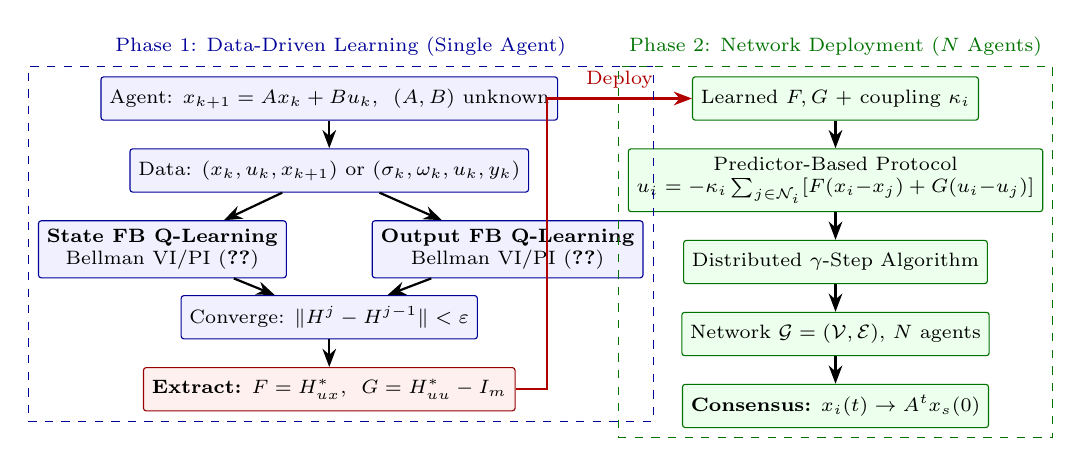
\begin{tikzpicture}[font=\scriptsize,
  box/.style={draw, rounded corners=1pt, align=center, inner sep=3pt, minimum height=5.5mm},
  lbox/.style={box, fill=blue!6, draw=blue!60!black},
  rbox/.style={box, fill=green!7, draw=green!45!black},
  xbox/.style={box, fill=red!6, draw=red!60!black},
  arr/.style={-Stealth, thick}]
% Phase 1
\node[lbox] (agent) {Agent: $x_{k+1}=Ax_k+Bu_k$,\ \ $(A,B)$ unknown};
\node[lbox, below=3.5mm of agent] (data) {Data: $(x_k,u_k,x_{k+1})$\ or\ $(\sigma_k,\omega_k,u_k,y_k)$};
\node[lbox, below left=3.5mm and -20mm of data] (sfq) {\textbf{State FB Q-Learning}\\ Bellman VI/PI \eqref{eq:bellman_vec}};
\node[lbox, below right=3.5mm and -20mm of data] (ofq) {\textbf{Output FB Q-Learning}\\ Bellman VI/PI \eqref{eq:ofb_bellman}};
\node[lbox, below=13mm of data] (convg) {Converge: $\|H^j-H^{j-1}\|<\varepsilon$};
\node[xbox, below=3.5mm of convg] (extract) {\textbf{Extract:} $F=H^*_{ux}$,\ \ $G=H^*_{uu}-I_m$};
\draw[arr] (agent) -- (data);
\draw[arr] (data) -- (sfq);
\draw[arr] (data) -- (ofq);
\draw[arr] (sfq) -- (convg);
\draw[arr] (ofq) -- (convg);
\draw[arr] (convg) -- (extract);
% Phase 2
\node[rbox, right=17mm of agent] (gains) {Learned $F,G$ + coupling $\kappa_i$};
\node[rbox, below=3.5mm of gains] (proto) {Predictor-Based Protocol\\ $u_i=-\kappa_i\sum_{j\in\mathcal N_i}[F(x_i{-}x_j)+G(u_i{-}u_j)]$};
\node[rbox, below=3.5mm of proto] (dist) {Distributed $\gamma$-Step Algorithm};
\node[rbox, below=3.5mm of dist] (net) {Network $\mathcal G=(\mathcal V,\mathcal E)$,\ $N$ agents};
\node[rbox, below=3.5mm of net] (cons) {\textbf{Consensus:} $x_i(t)\to A^t x_s(0)$};
\draw[arr] (gains) -- (proto);
\draw[arr] (proto) -- (dist);
\draw[arr] (dist) -- (net);
\draw[arr] (net) -- (cons);
\draw[arr, red!70!black] (extract.east) -| ++(4mm,0) |- node[pos=0.75, above]{\textcolor{red!70!black}{Deploy}} (gains.west);
\node[draw=blue!60!black, dashed, fit=(agent)(data)(sfq)(ofq)(convg)(extract), inner sep=3.5pt,
      label={[blue!60!black]above:{\scriptsize Phase 1: Data-Driven Learning (Single Agent)}}] {};
\node[draw=green!45!black, dashed, fit=(gains)(proto)(dist)(net)(cons), inner sep=3.5pt,
      label={[green!45!black]above:{\scriptsize Phase 2: Network Deployment ($N$ Agents)}}] {};
\end{tikzpicture}}
\caption{Proposed data-driven methodology. Phase~1: offline Q-learning on a single agent to extract consensus gains $F$ and $G$. Phase~2: deployment in the predictor-based protocol across the multi-agent network.}
\label{fig:block_diagram}
\end{figure*}
\subsection{State Feedback Q-Learning}
\label{sec:sf_ql}
For a single agent~\eqref{eq:agent_state} with weights $(Q,R)$ under a stabilizing policy $u_k = -Kx_k$, the cost-to-go is $V(x_k) = x_k^\top P_K x_k$, and the Q-function---the cost of an arbitrary $u_k$ now, following the policy afterwards---is
\begin{equation}
Q_K(x_k,u_k) = x_k^\top Q x_k + u_k^\top R u_k + x_{k+1}^\top P_K\, x_{k+1},
\label{eq:qdef}
\end{equation}
with $x_{k+1} = Ax_k + Bu_k$, which collects into a quadratic form in $z_k = [x_k^\top\; u_k^\top]^\top$. Partitioning the kernel conformably with $z_k$,
\begin{equation}
Q_K = z_k^\top H z_k, \qquad
H = \begin{bmatrix} H_{xx} & H_{xu} \\ H_{ux} & H_{uu} \end{bmatrix},
\label{eq:Hpartition}
\end{equation}
whose blocks carry the model:
\begin{equation}
\begin{bmatrix} H_{xx} & H_{xu} \\ H_{ux} & H_{uu} \end{bmatrix}
= \begin{bmatrix} Q + A^\top\! PA & A^\top\! PB \\ B^\top\! PA & R + B^\top\! PB \end{bmatrix},
\label{eq:Hmatrix}
\end{equation}
with optimal policy $u_k^* = -(H_{uu}^*)^{-1}H_{ux}^* x_k$~\cite{bradtke1994}. The bottom blocks of~\eqref{eq:Hmatrix} are, up to $R$, exactly the matrices of~\eqref{eq:FG_dare}. The match is exact at the optimal $P$ under one condition: the LQR DARE
\begin{equation}
A^\top\! PA - P + Q - A^\top\! PB(R + B^\top\! PB)^{-1}B^\top\! PA = 0
\label{eq:dare_lqr}
\end{equation}
coincides with the consensus DARE~\eqref{eq:dare} if and only if $R = I_m$. The weight $R = I_m$ is thus forced, not chosen, and yields the bridge on which the paper rests.
\begin{lemma}[Consensus gains from the Q-kernel]
\label{prop:FG_recovery}
Let $H^*$ be the optimal H-matrix of the LQR problem with weights $(Q, I_m)$. Then
\begin{equation}
F = H_{ux}^*, \qquad G = H_{uu}^* - I_m.
\label{eq:FG_from_H}
\end{equation}
\end{lemma}
\begin{proof}
Under the optimal value $V^*(x_k) = x_k^\top P^* x_k$ and $R = I_m$, the Q-function~\eqref{eq:qdef} expands as
\begin{align}
Q^*(x_k,u_k)
&= x_k^\top Q x_k + u_k^\top u_k \notag\\
&\quad + (Ax_k + Bu_k)^\top P^* (Ax_k + Bu_k) \notag\\
&= \begin{bmatrix} x_k\\ u_k\end{bmatrix}^{\!\top}\!
\begin{bmatrix} Q + A^\top\! P^* A & A^\top\! P^* B\\ B^\top\! P^* A & I_m + B^\top\! P^* B\end{bmatrix}\!
\begin{bmatrix} x_k\\ u_k\end{bmatrix}.
\end{align}
Reading off the lower blocks and comparing with~\eqref{eq:FG_dare},
\begin{align}
H_{ux}^* &= B^\top P^* A = F,\\
H_{uu}^* &= I_m + B^\top P^* B = I_m + G,
\end{align}
which is~\eqref{eq:FG_from_H}.
\end{proof}
\begin{remark}[Layout versus numbers]
\label{rem:layout}
Lemma~\ref{prop:FG_recovery} locates the gains inside $H^*$ but provides no numerical entry of it: \eqref{eq:Hmatrix} is written in the unknown $(A,B,P)$. The entries are obtained from data by~\eqref{eq:bellman_consensus}--\eqref{eq:vi_update} below. Note also that standard Q-learning compresses $H^*$ into the regulator $K^* = (I_m+G)^{-1}F$---precisely the limit matrix in~\eqref{eq:limit}---and discards the blocks; deploying $K^*$ would drive every agent to the origin. Consensus requires the raw blocks, never the regulator.
\end{remark}
Along any measured trajectory with $R = I_m$, the kernel $H$ satisfies the Bellman equation
\begin{equation}
z_k^\top H z_k = x_k^\top Q x_k + u_k^\top u_k + z_{k+1}^\top H z_{k+1},
\label{eq:bellman_consensus}
\end{equation}
in which every quantity except $H$ is measured; \eqref{eq:bellman_consensus} is an equation whose unknown is $H$ itself, and it is here---not in Lemma~\ref{prop:FG_recovery}---that the model is replaced by data.

To see how~\eqref{eq:bellman_consensus} operates on data, write the quadratic form as an inner product~\cite[Sec.~2.4]{rizvi2022}. With $z_k \in \R^{l}$, $l = n+m$, define the quadratic data vector and the vectorized kernel
\begin{align}
\bar{z}_k &= \big[z_{k,1}^2,\; z_{k,1}z_{k,2},\; \ldots,\; z_{k,1}z_{k,l},\; z_{k,2}^2,\; \ldots,\; z_{k,l}^2\big]^\top, \label{eq:zbar}\\
\bar{H} &= \vecs(H) = \big[h_{11},\, 2h_{12},\, \ldots,\, 2h_{1l},\, h_{22},\, \ldots,\, h_{ll}\big]^\top, \label{eq:vecsH}
\end{align}
both in $\R^{l(l+1)/2}$, so that $z_k^\top H z_k = \bar{H}^\top \bar{z}_k$ identically (the factor $2$ on the off-diagonal entries absorbs the symmetry of $H$). Each time step then contributes one linear equation in the unknown $\bar{H}$,
\begin{equation}
\bar{H}^\top (\bar{z}_k - \bar{z}_{k+1}) = x_k^\top Q x_k + u_k^\top u_k \eqqcolon r_k,
\label{eq:bellman_vec}
\end{equation}
and stacking $N_d$ consecutive samples,
\begin{equation}
\Phi = \begin{bmatrix} (\bar{z}_0 - \bar{z}_1)^\top \\ \vdots \\ (\bar{z}_{N_d-1} - \bar{z}_{N_d})^\top \end{bmatrix}\!, \quad
\Psi = \begin{bmatrix} r_0 \\ \vdots \\ r_{N_d-1} \end{bmatrix}\!,
\label{eq:PhiPsi}
\end{equation}
yields the batch least-squares solution
\begin{equation}
\bar{H} = (\Phi^\top \Phi)^{-1} \Phi^\top \Psi,
\label{eq:ls_solve}
\end{equation}
valid when $\rank(\Phi) = l(l+1)/2$, which requires $N_d \geq l(l+1)/2$ sufficiently different samples. The probing input $u_k = -K^j x_k + e_k$ supplies this rank and, entering $z_k$ and $z_{k+1}$ symmetrically, cancels from~\eqref{eq:bellman_vec} without bias~\cite{bradtke1994,rizvi2022}. A single regression~\eqref{eq:ls_solve} evaluates the current policy; the optimal $H^*$ is reached by iterating. PI solves~\eqref{eq:PhiPsi}--\eqref{eq:ls_solve} and updates $K^{j+1} = (H_{uu}^j)^{-1} H_{ux}^j$; VI replaces the rows of $\Phi$ by $\bar{z}_k^\top$ and the targets by $r_k + (\bar{H}^j)^\top \bar{z}_{k+1}$, i.e., it solves
\begin{equation}
(\bar{H}^{j+1})^\top \bar{z}_k = x_k^\top Q x_k + u_k^\top u_k + (\bar{H}^j)^\top \bar{z}_{k+1},
\label{eq:vi_update}
\end{equation}
and converges from $H^0 = 0$---the natural choice here, since the plants are open-loop unstable and no stabilizing initial policy is available. Upon convergence, $F = H_{ux}^*$ and $G = H_{uu}^* - I_m$. Because the DARE depends only on $(A,B,Q)$ and not on the graph, the learning runs on one agent and the gains deploy across all $N$; the learning cost is independent of the network size, and the implicit coupling of~\eqref{eq:protocol} never enters the learning phase.
\begin{theorem}[State feedback convergence and consensus]
\label{thm:sf_convergence}
Let Assumptions~\ref{ass:controllable} and~\ref{ass:graph} hold, let $(A, \sqrt{Q})$ be observable, and let the rank condition $\rank(\Phi) = l(l+1)/2$ hold at every iteration. Then:
\begin{enumerate}
    \item[(i)] The Q-learning iterations converge: $H^j \to H^*$ as $j \to \infty$.
    \item[(ii)] The extracted gains $F = H_{ux}^*$ and $G = H_{uu}^* - I_m$ satisfy~\eqref{eq:FG_dare}.
    \item[(iii)] The protocol~\eqref{eq:protocol} with Q-learned gains achieves (multi-)consensus if $\kappa_i \bar{r} > 1$.
    \item[(iv)] Exploration noise does not bias the learned H-matrix.
\end{enumerate}
\end{theorem}
\begin{proof}
\emph{(i) Convergence.} Under the rank condition, the least-squares solutions of~\eqref{eq:bellman_vec} and~\eqref{eq:vi_update} coincide with the exact recursions they encode. With $R = I_m$, PI alternates policy evaluation and improvement,
\begin{align}
P^j &= Q + (K^j)^\top K^j + (A - BK^j)^\top P^j (A - BK^j), \label{eq:pi_eval}\\
K^{j+1} &= (I_m + B^\top P^j B)^{-1} B^\top P^j A, \label{eq:pi_improve}
\end{align}
which is Hewer's algorithm: $P^j$ decreases monotonically to the unique stabilizing solution $P^*$ of~\eqref{eq:dare}, with $A - BK^j$ Schur at every step~\cite{hewer1971}. VI encodes the Riccati difference recursion
\begin{equation}
P^{j+1} = Q + A^\top\! P^j A - A^\top\! P^j B (I_m + B^\top\! P^j B)^{-1} B^\top\! P^j A,
\label{eq:vi_riccati}
\end{equation}
which converges to $P^*$ from any $P^0 \geq 0$ when $(A, \sqrt{Q})$ is observable~\cite{lewis2009,rizvi2022}. In either case the reconstructed kernel converges,
\begin{equation}
H^j = \begin{bmatrix} Q + A^\top\! P^j A & A^\top\! P^j B\\ B^\top\! P^j A & I_m + B^\top\! P^j B\end{bmatrix} \longrightarrow H^*.
\end{equation}
\emph{(ii) Exact gain recovery.} By Lemma~\ref{prop:FG_recovery}, the converged blocks are
\begin{equation}
F = H_{ux}^* = B^\top\! P^* A, \qquad G = H_{uu}^* - I_m = B^\top\! P^* B,
\end{equation}
and since $P^*$ solves~\eqref{eq:dare}, these coincide exactly with~\eqref{eq:FG_dare}---an equality, not an approximation.
\emph{(iii) Consensus.} Because $F$ and $G$ satisfy~\eqref{eq:FG_dare}, the design condition of~\cite[Thm.~3.1]{cacace2024}, extended to $Q = C^\top Q_y C \succeq 0$ by Lemma~\ref{lem:psdQ}, applies: the modes~\eqref{eq:spectrum} are Schur for every nonzero $\bar{\lambda}_k$ under~\eqref{eq:coupling}. For $\mu > 1$ reaches, the block-triangular structure~\eqref{eq:L_block} drives the agents in each cell of $\pi^\star$ to a common trajectory~\cite[Thm.~4.1]{cacace2024}.
\emph{(iv) Noise immunity.} Under $u_k = -K^j x_k + e_k$ the successor state is
\begin{equation}
x_{k+1} = (A - BK^j)x_k + B e_k,
\end{equation}
so $e_k$ enters $z_k$ and $z_{k+1}$ symmetrically and cancels in~\eqref{eq:bellman_vec}; the least-squares solution equals the noise-free one whenever the rank condition holds~\cite{bradtke1994,rizvi2022}.
\end{proof}
The complete procedure is summarized in Algorithm~\ref{alg:sf_ql}.
\begin{algorithm}[!htb]
\caption{State Feedback Q-Learning for Consensus Gains}
\label{alg:sf_ql}
{\footnotesize
\begin{algorithmic}[1]
\REQUIRE System order $n$, input dimension $m$; cost matrix $Q = C^\top Q_y C$; tolerance $\varepsilon > 0$.
\ENSURE Consensus gains $F \in \R^{m \times n}$, $G \in \R^{m \times m}$.
\STATE Set $R = I_m$, $l = n + m$, $N_p = l(l+1)/2$; define $E_x = [\,I_n \;\; 0\,]$, $E_u = [\,0 \;\; I_m\,]$.
\STATE Initialize $K^0$ (stabilizing for PI; zero for VI); $\bar{H}^0 = \vecs(I_l)$, $j \leftarrow 0$.
\REPEAT
    \FOR{$k = 0, 1, \ldots, N_d-1$ where $N_d \geq N_p$}
        \STATE Apply $u_k = -K^j x_k + e_k$, measure $x_{k+1}$
        \STATE Form $z_k = [x_k^\top \;\; u_k^\top]^\top$; compute $\bar{z}_k$ from unique elements of $z_k z_k^\top$
        \STATE Compute stage cost $r_k = x_k^\top Q x_k + u_k^\top u_k$
    \ENDFOR
    \STATE \textbf{PI:} rows $(\bar{z}_k - \bar{z}_{k+1})^\top$, targets $r_k$; solve $\Phi \bar{H}^j = \Psi$
    \STATE \textbf{VI:} rows $\bar{z}_k^\top$, targets $r_k + (\bar{H}^j)^\top \bar{z}_{k+1}$; solve $\Phi \bar{H}^{j+1} = \Psi$
    \STATE Reshape $\bar{H} \to H$ (symmetric); $H_{ux} = E_u H E_x^\top$, $H_{uu} = E_u H E_u^\top$
    \STATE $K^{j+1} = (H_{uu}^j)^{-1} H_{ux}^j$, \; $j \leftarrow j + 1$
\UNTIL{$\|\bar{H}^j - \bar{H}^{j-1}\| < \varepsilon$}
\STATE \textbf{return} $F = H_{ux}^*$, \; $G = H_{uu}^* - I_m$
\end{algorithmic}}
\end{algorithm}
\subsection{Output Feedback Q-Learning}
\label{sec:ofb_ql}
When only $y_i = Cx_i$ is measurable, the protocol~\eqref{eq:protocol} cannot be evaluated (it needs $F(x_i - x_j)$) and the data $z_k = (x_k,u_k)$ of Section~\ref{sec:sf_ql} is unavailable. An observer would repair both but requires $(A,B,C)$; identification would defeat the purpose. The state must be recovered without the model.

Under Assumption~\ref{ass:observable}, choose $L$ such that $A + LC$ is Schur and rewrite~\eqref{eq:agent_state} with the output injection $L y_k$:
\begin{equation}
x_{k+1} = (A + LC)x_k + Bu_k - L y_k.
\label{eq:obs_rewrite}
\end{equation}
Unrolling~\eqref{eq:obs_rewrite} expresses the state through the input-output history,
\begin{equation}
x_k = \sum_{i=0}^{k-1}(A+LC)^{k-1-i}\big(Bu_i - L y_i\big) + (A+LC)^k x_0,
\label{eq:unrolled}
\end{equation}
whose sums are computed recursively by two filter banks driven by the inputs and outputs,
\begin{equation}
\sigma_{k+1}^i = \mathcal{A}\sigma_k^i + \mathcal{B}u_k^i, \qquad \omega_{k+1}^i = \mathcal{A}\omega_k^i + \mathcal{B}y_k^i,
\label{eq:filters}
\end{equation}
with $\mathcal{A}$ a companion matrix carrying the eigenvalues of $A + LC$ and $\mathcal{B} = [1 \, 0 \cdots 0]^\top$, so that~\eqref{eq:unrolled} takes the compact form~\cite[Thm.~2.1]{rizvi2022}
\begin{equation}
x_k = W_u \sigma_k + W_y \omega_k + (A + LC)^k x_0
\label{eq:state_param}
\end{equation}
for fixed $W_u \in \R^{n \times mn}$, $W_y \in \R^{n \times pn}$ built from the unknown model---matrices that are never computed in what follows. Placing all eigenvalues of $\mathcal{A}$ at the origin (dead-beat) gives $(A+LC)^n = 0$, hence~\cite[Thm.~2.2]{rizvi2022}
\begin{equation}
x_k = W_u \sigma_k + W_y \omega_k \qquad \text{exactly, for all } k \geq n,
\label{eq:deadbeat}
\end{equation}
and $W = [W_u \; W_y]$ has full row rank when $A$ has no zero eigenvalue~\cite[Thm.~2.4, Rem.~2.2]{rizvi2022}. The exactness of~\eqref{eq:deadbeat} propagates through everything below.

Substituting~\eqref{eq:deadbeat} into~\eqref{eq:Hmatrix} with $R = I_m$ converts the Q-function into a quadratic form in the measurable $\tilde{z}_k = [\,\sigma_k^\top \;\; \omega_k^\top \;\; u_k^\top\,]^\top$:
\begin{align}
Q_K &= x^\top(Q + A^\top\! PA)x + 2\,x^\top\!(A^\top\! PB)\,u \notag\\
&\quad + u^\top(I_m + B^\top\! PB)\,u \notag\\
&= \tilde{z}_k^\top \tilde{H} \tilde{z}_k, \qquad \tilde{l} = mn + pn + m.
\label{eq:ofb_qfunc}
\end{align}
Partitioning $\tilde{H}$ conformably with $\tilde{z}_k = [\,\sigma_k^\top \; \omega_k^\top \; u_k^\top\,]^\top$,
\begin{equation}
\tilde{H} = \begin{bmatrix}
\tilde{H}_{\sigma\sigma} & \tilde{H}_{\sigma\omega} & \tilde{H}_{\sigma u} \\
\tilde{H}_{\omega\sigma} & \tilde{H}_{\omega\omega} & \tilde{H}_{\omega u} \\
\tilde{H}_{u\sigma} & \tilde{H}_{u\omega} & \tilde{H}_{uu}
\end{bmatrix},
\label{eq:Htilde_partition}
\end{equation}
the substitution shows that the cross blocks pick up the parameterization matrices while the input-input block does not:
\begin{align}
\tilde{H}_{u\sigma} &= B^\top\! P A\, W_u = F W_u, \notag\\
\tilde{H}_{u\omega} &= B^\top\! P A\, W_y = F W_y, \label{eq:ofb_blocks}\\
\tilde{H}_{uu} &= I_m + B^\top\! P B, \notag
\end{align}
(the upper blocks, e.g.\ $\tilde{H}_{\sigma\sigma} = W_u^\top(Q + A^\top\! PA)W_u$, are not needed by the protocol and are listed only through~\eqref{eq:Htilde_partition}).
Equation~\eqref{eq:ofb_blocks} contains the central tension of output feedback: the learner never sees $F$ alone---only $FW_u$ and $FW_y$, entangled with unknown matrices---while $\tilde{H}_{uu}$ carries no $W$ factor, so $G$ is always exact. As in Remark~\ref{rem:layout}, \eqref{eq:ofb_blocks} is only the layout of $\tilde{H}$; its entries come from the Bellman equation on the measurable triple, with the cost on outputs~\cite[Eq.~(2.27)]{rizvi2022},
\begin{equation}
\tilde{z}_k^\top \tilde{H} \tilde{z}_k = y_k^\top Q_y y_k + u_k^\top u_k + \tilde{z}_{k+1}^\top \tilde{H} \tilde{z}_{k+1}.
\label{eq:ofb_bellman}
\end{equation}
The machinery of~\eqref{eq:zbar}--\eqref{eq:ls_solve} operates verbatim on the extended vector: the quadratic data vector $\bar{\tilde{z}}_k \in \R^{\tilde{l}(\tilde{l}+1)/2}$ and the vectorized kernel $\bar{\tilde{H}} = \vecs(\tilde{H})$ are built from $\tilde{z}_k$ exactly as in~\eqref{eq:zbar}--\eqref{eq:vecsH}, giving $\tilde{z}_k^\top \tilde{H} \tilde{z}_k = \bar{\tilde{H}}^\top \bar{\tilde{z}}_k$, and the VI regression
\begin{equation}
(\bar{\tilde{H}}^{j+1})^\top \bar{\tilde{z}}_k = y_k^\top Q_y y_k + u_k^\top u_k + (\bar{\tilde{H}}^{j})^\top \bar{\tilde{z}}_{k+1}
\label{eq:of_vi}
\end{equation}
is solved in batch from $N_d \geq \tilde{l}(\tilde{l}+1)/2$ samples, with the same rank condition and the same noise-cancellation structure. Convergence yields a numeric table $\tilde{H}^*$ whose blocks are obtained without ever knowing the $F$, $W_u$, $W_y$ they are made of. (The optimal law $u_k^* = -(\tilde{H}_{uu}^*)^{-1}(\tilde{H}_{u\sigma}^* \sigma_k + \tilde{H}_{u\omega}^* \omega_k)$ of~\cite[Thm.~2.5]{rizvi2022} is the absolute regulator in disguise and is not deployed, per Remark~\ref{rem:layout}.)

The converged table thus provides $\tilde{H}_{u\sigma}^* = FW_u$ and $\tilde{H}_{u\omega}^* = FW_y$, while the protocol needs $F(x_i - x_j)$---and neither $F$, nor $W_u,W_y$, nor $x_i$ is separately known. The following result, the central one of the paper, shows that no separation is needed.
\begin{proposition}[Output-feedback disagreement reconstruction]
\label{prop:disagreement}
Let $\tilde{H}^*$ be the converged output-feedback Q-matrix with blocks~\eqref{eq:ofb_blocks} evaluated at $P^*$, and let all agents run identical filters~\eqref{eq:filters}. Then the predictor coupling gain is recovered as
\begin{equation}
G = \tilde{H}_{uu}^* - I_m = B^\top P^* B,
\label{eq:G_ofb}
\end{equation}
and, for any agents $i,j$ and all $k \geq n$ under the dead-beat parameterization, the state-disagreement feedback in~\eqref{eq:protocol} is reconstructed from the filter states as
\begin{equation}
F(x_i - x_j) = \tilde{H}_{u\sigma}^*(\sigma_i - \sigma_j) + \tilde{H}_{u\omega}^*(\omega_i - \omega_j).
\label{eq:disagreement}
\end{equation}
\end{proposition}
\begin{proof}
The gain~\eqref{eq:G_ofb} is immediate from $\tilde{H}_{uu}^* = I_m + B^\top P^* B$ in~\eqref{eq:ofb_blocks}. For~\eqref{eq:disagreement}: because every agent runs the identical filters~\eqref{eq:filters}, the same $W_u$, $W_y$ describe every agent, so the dead-beat identity~\eqref{eq:deadbeat} applied to agents $i$ and $j$ gives, for $k \geq n$,
\begin{align}
x_i &= W_u \sigma_i + W_y \omega_i,\\
x_j &= W_u \sigma_j + W_y \omega_j,
\end{align}
and, by linearity,
\begin{equation}
x_i - x_j = W_u(\sigma_i - \sigma_j) + W_y(\omega_i - \omega_j).
\end{equation}
Premultiplying by $F$ and substituting $\tilde{H}_{u\sigma}^* = F W_u$ and $\tilde{H}_{u\omega}^* = F W_y$ from~\eqref{eq:ofb_blocks},
\begin{align}
F(x_i - x_j) &= F W_u(\sigma_i - \sigma_j) + F W_y(\omega_i - \omega_j) \notag\\
&= \tilde{H}_{u\sigma}^*(\sigma_i - \sigma_j) + \tilde{H}_{u\omega}^*(\omega_i - \omega_j),
\end{align}
which is~\eqref{eq:disagreement}.
\end{proof}
The protocol never needed $F$: it needs $F$ times a difference, and~\eqref{eq:disagreement} expresses that entirely through the numeric blocks. Each agent therefore deploys the predictor protocol from output data,
\begin{align}
u_i = -\kappa_i \sum_{j \in \mathcal{N}_i} \big[ &\tilde{H}_{u\sigma}^*(\sigma_i - \sigma_j) + \tilde{H}_{u\omega}^*(\omega_i - \omega_j) \notag\\
&+ G(u_i - u_j) \big],
\label{eq:ofb_deploy}
\end{align}
with neighbors exchanging $(\sigma_j, \omega_j, u_j)$ in place of states and $u_i = 0$ during the first $n$ steps while the filters fill. The complete per-step operation of agent $i$ at time $t$ is thus:
\begin{enumerate}
\item[1)] update its own filters $\sigma_i, \omega_i$ by~\eqref{eq:filters} from its own $(u_i, y_i)$;
\item[2)] exchange $(\sigma_j, \omega_j, u_j)$ with its in-neighbors $j \in \mathcal{N}_i$;
\item[3)] form the reconstructed disagreement $\tilde{H}_{u\sigma}^*(\sigma_i - \sigma_j) + \tilde{H}_{u\omega}^*(\omega_i - \omega_j)$ of~\eqref{eq:disagreement};
\item[4)] resolve the implicit coupling by the $\gamma$-step rounds~\eqref{eq:dist_init}--\eqref{eq:dist_iter}, with the reconstruction in place of $F(x_i - x_j)$, and apply $u_i(t) = v_i(t,\gamma)$.
\end{enumerate}
Every quantity in steps 1)--4) is either a learned block of $\tilde{H}^*$ or a measured signal. Because~\eqref{eq:disagreement} is an identity, the network under~\eqref{eq:ofb_deploy} traces the same trajectories as the state feedback deployment. Fig.~\ref{fig:of_prop1} verifies both halves numerically: the reconstruction error collapses to numerical zero precisely at $k = n$, and across all three scenarios of Section~\ref{sec:results} the output-feedback trajectories coincide with their state-feedback counterparts to within $10^{-11}$.
\begin{figure*}[!t]
    \centering
    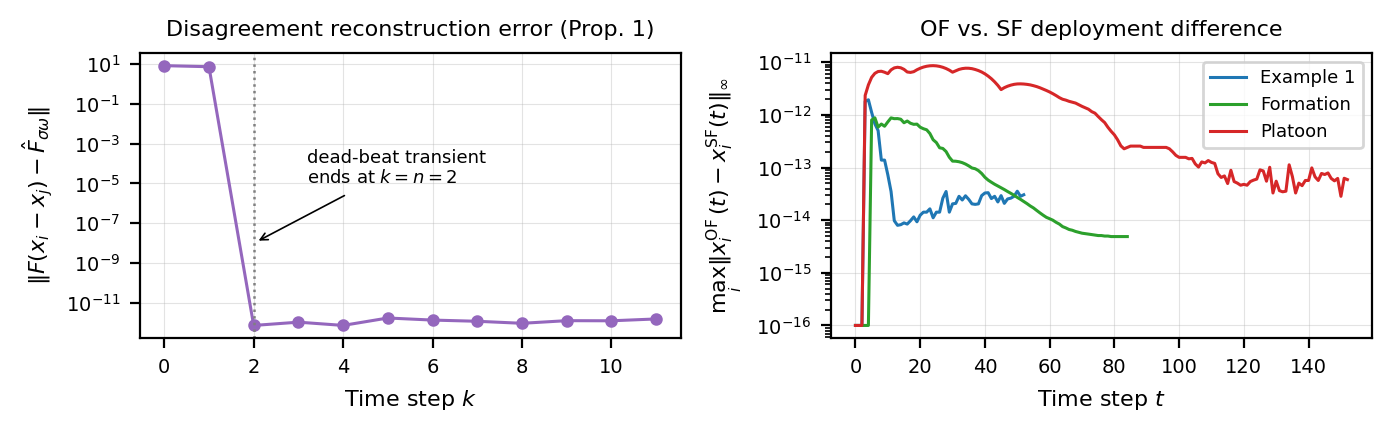
\includegraphics[width=0.9\textwidth]{fig_of_prop1.png}
    \caption{Numerical evidence for Proposition~\ref{prop:disagreement}. Left: disagreement reconstruction error along a two-agent trajectory (Example 1 system); the error is exactly zero for $k \geq n = 2$. Right: maximum deviation between output-feedback and state-feedback network deployments for all three scenarios of Section~\ref{sec:results}.}
    \label{fig:of_prop1}
\end{figure*}
\begin{theorem}[Output feedback convergence and consensus]
\label{thm:ofb_convergence}
Let Assumptions~\ref{ass:controllable}--\ref{ass:graph} hold, with $(A, \sqrt{Q})$ observable, $W$ of full row rank, and the excitation rank condition satisfied at every iteration. Then:
\begin{enumerate}
\item[(i)] $\tilde{H}^j \to \tilde{H}^*$;
\item[(ii)] $G = \tilde{H}_{uu}^* - I_m = B^\top P^*B$ and the disagreement feedback~\eqref{eq:disagreement} is recovered;
\item[(iii)] the protocol~\eqref{eq:ofb_deploy} achieves (multi-)consensus under $\kappa_i \bar{r} > 1$;
\item[(iv)] the scheme is immune to exploration noise bias.
\end{enumerate}
\end{theorem}
\begin{proof}
\emph{(i) Convergence.} Substituting the steady-state parameterization $x_k = W_u\sigma_k + W_y\omega_k$ into the output-feedback Bellman equation~\eqref{eq:ofb_bellman} and collecting terms with $W = [W_u\ W_y]$ gives
\begin{align}
W^\top P^j W = W^\top\big(&Q + (K^j)^\top K^j \notag\\
&+ (A - BK^j)^\top P^j (A - BK^j)\big) W.
\label{eq:W_sandwich}
\end{align}
Since $W$ has full row rank, $WW^\top \succ 0$; pre-multiplying~\eqref{eq:W_sandwich} by $(WW^\top)^{-1}W$ and post-multiplying by $W^\top(WW^\top)^{-1}$ cancels $W$ on both sides and recovers the state-feedback evaluation~\eqref{eq:pi_eval},
\begin{equation}
P^j = Q + (K^j)^\top K^j + (A - BK^j)^\top P^j (A - BK^j),
\end{equation}
so the iterations coincide with the recursions of Theorem~\ref{thm:sf_convergence} and $P^j \to P^*$~\cite[Thms.~2.6, 2.7]{rizvi2022}. The reconstructed blocks
\begin{align}
\tilde{H}_{u\sigma}^j &= B^\top\! P^j A\, W_u, \qquad
\tilde{H}_{u\omega}^j = B^\top\! P^j A\, W_y, \notag\\
\tilde{H}_{uu}^j &= I_m + B^\top\! P^j B
\end{align}
therefore converge to $\tilde{H}^*$ as $P^j \to P^*$.
\emph{(ii) Gain and disagreement recovery.} From the converged blocks,
\begin{align}
G &= \tilde{H}_{uu}^* - I_m = B^\top\! P^* B,\\
F(x_i - x_j) &= \tilde{H}_{u\sigma}^*(\sigma_i - \sigma_j) + \tilde{H}_{u\omega}^*(\omega_i - \omega_j),
\end{align}
the second line by Proposition~\ref{prop:disagreement}, so the protocol~\eqref{eq:ofb_deploy} is realized entirely from input-output data.
\emph{(iii) Consensus.} With $\tilde{H}_{u\sigma}^* = B^\top P^* A W_u$ and $\tilde{H}_{uu}^* = I_m + B^\top P^* B$ for $P^*$ solving~\eqref{eq:dare}, the deployed gains equal~\eqref{eq:FG_dare}, so by Lemma~\ref{lem:psdQ} the closed-loop modes~\eqref{eq:spectrum} are Schur for every nonzero $\bar{\lambda}_k$ under~\eqref{eq:coupling}, exactly as in Theorem~\ref{thm:sf_convergence}(iii).
\emph{(iv) Noise immunity.} The extended Bellman equation~\eqref{eq:ofb_bellman} has the same symmetric structure in $e_k$ as~\eqref{eq:bellman_consensus}, so the scheme inherits the bias-free property of~\cite[Thm.~2.8]{rizvi2022}.
\end{proof}
\begin{algorithm}[!htb]
\caption{Output Feedback Q-Learning for Consensus Gains}
\label{alg:ofb_ql}
{\footnotesize
\begin{algorithmic}[1]
\REQUIRE System order $n$, dimensions $m$, $p$; cost $Q_y \geq 0$; tolerance $\varepsilon$.
\ENSURE Gain $G$ and disagreement blocks $\tilde{H}_{u\sigma}^*$, $\tilde{H}_{u\omega}^*$.
\STATE Set $R = I_m$, $\tilde{l} = mn + pn + m$, $\tilde{N}_p = \tilde{l}(\tilde{l}+1)/2$.
\STATE Choose companion $\mathcal{A}$ (all eigenvalues zero for dead-beat), $\mathcal{B} = [1 \; 0 \; \cdots \; 0]^\top$.
\STATE Initialize $\bar{\tilde{H}}^0$, $\bar{K}^0 = 0$, $j \leftarrow 0$; $\sigma_0^i = 0$, $\omega_0^i = 0$.
\FOR{$k = 0, 1, \ldots, N_d-1$}
    \STATE Apply $u_k = -\bar{K}^j [\sigma_k^\top \; \omega_k^\top]^\top + e_k$, measure $y_k$; update filters via~\eqref{eq:filters}
    \STATE Form $\tilde{z}_k = [\sigma_k^\top \; \omega_k^\top \; u_k^\top]^\top$, $\bar{\tilde{z}}_k$, and $r_k = y_k^\top Q_y y_k + u_k^\top u_k$
\ENDFOR
\REPEAT
    \STATE \textbf{VI:} rows $\bar{\tilde{z}}_k^\top$, targets $r_k + (\bar{\tilde{H}}^j)^\top \bar{\tilde{z}}_{k+1}$; solve $\tilde{\Phi} \bar{\tilde{H}}^{j+1} = \tilde{\Psi}$
    \STATE Reshape; $\bar{K}^{j+1} = (\tilde{H}_{uu}^{j+1})^{-1} [\tilde{H}_{u\sigma}^{j+1} \;\; \tilde{H}_{u\omega}^{j+1}]$, \; $j \leftarrow j + 1$
\UNTIL{$\|\bar{\tilde{H}}^j - \bar{\tilde{H}}^{j-1}\| < \varepsilon$}
\STATE $G = \tilde{H}_{uu}^* - I_m$; deploy~\eqref{eq:ofb_deploy} using~\eqref{eq:disagreement} after an $n$-step filter warm-up.
\end{algorithmic}}
\end{algorithm}
%% ===================================================================
\section{Results}
\label{sec:results}
%% ===================================================================
We validate the approach on two scenarios adapted from~\cite{cacace2024}---multi-leader following ($N{=}9$) and formation control ($N{=}6$, $T = 0.1$~s)---together with a robustness study and a vehicle-platoon example. Every scenario is executed under \emph{both} state feedback and output feedback, and validation is performed by direct comparison with the model-based design of~\cite{cacace2024}: the Q-learned gains are checked for exact numerical agreement with the DARE solution, and the output-feedback deployment is checked for exact agreement with the state-feedback deployment (Proposition~\ref{prop:disagreement}). All simulations use $R = I_m$ and VI, and the output-feedback runs employ the $n$-step dead-beat filter warm-up of Section~\ref{sec:ofb_ql}.
\subsection{Example 1: Multi-Leader Following ($N = 9$, $\mu = 3$)}
\label{subsec:sim1}
We consider $N = 9$ agents with sampled double integrator dynamics ($T = 1$)
\begin{equation}
A = \begin{bmatrix} 1 & 1 \\ 0 & 1 \end{bmatrix}, \quad
B = \begin{bmatrix} T^2/2 \\ T \end{bmatrix} = \begin{bmatrix} 0.5 \\ 1 \end{bmatrix}, \quad
C = \begin{bmatrix} 1 & 0 \end{bmatrix},
\label{eq:AB_ex1}
\end{equation}
communicating over the digraph in Fig.~\ref{fig:graph9}. Nodes 1, 2, and 3 have no in-neighbors and are therefore genuine roots: the graph has $\mu = 3$ reaches with exclusive parts $\mathcal{H}_k = \{k\}$, $k = 1,2,3$, and common part $\mathcal{C} = \{4,\ldots,9\}$. The coarsest AEP has $p = 4$ common cells,
\begin{equation*}
\mathcal{C}_{\mu+1} = \{4,5,6\}, \quad \mathcal{C}_{\mu+2} = \{7\}, \quad \mathcal{C}_{\mu+3} = \{8\}, \quad \mathcal{C}_{\mu+4} = \{9\},
\end{equation*}
with mixing vectors $\gamma^{k}$ giving asymptotic leader weights $(\tfrac12,\tfrac12,0)$ for node 7, $(0,\tfrac12,\tfrac12)$ for node 8, $(\tfrac14,\tfrac12,\tfrac14)$ for node 9, and $(\tfrac18,\tfrac12,\tfrac38)$ for the cell $\{4,5,6\}$. The nonzero Laplacian eigenvalues are all equal to $2$, so $\bar{r} = 2$ and the choice $\kappa_i = 2$ gives $\kappa_i\bar{r} = 4 > 1$ with strict margin. We set $Q_y = 1$, hence $Q = C^\top Q_y C$, and $x_i(0) = i\ones_2$.
\begin{figure}[!htbp]
\centering
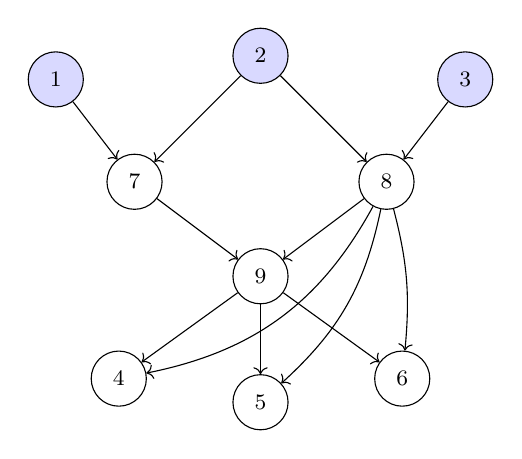
\begin{tikzpicture}[
    node distance=1.6cm,
    every node/.style={circle, draw, minimum size=0.7cm, font=\footnotesize},
    every edge/.style={draw, -Stealth, thick},
    leader/.style={fill=blue!15}
]
\node[leader] (1) at (-2.6, 2.3) {1};
\node[leader] (2) at (0, 2.6) {2};
\node[leader] (3) at (2.6, 2.3) {3};
\node (7) at (-1.6, 1.0) {7};
\node (8) at (1.6, 1.0) {8};
\node (9) at (0, -0.2) {9};
\node (4) at (-1.8, -1.5) {4};
\node (5) at (0, -1.8) {5};
\node (6) at (1.8, -1.5) {6};
\draw[->] (1) -- (7);
\draw[->] (2) -- (7);
\draw[->] (2) -- (8);
\draw[->] (3) -- (8);
\draw[->] (7) -- (9);
\draw[->] (8) -- (9);
\draw[->] (9) -- (4);
\draw[->] (9) -- (5);
\draw[->] (9) -- (6);
\draw[->] (8) to[bend left=25] (4);
\draw[->] (8) to[bend left=18] (5);
\draw[->] (8) to[bend left=10] (6);
\end{tikzpicture}
\caption{Communication digraph for Example~1 ($N=9$, $\mu=3$). Blue nodes are leaders (zero in-degree); each follower cell of the coarsest AEP receives a distinct convex mix of the leader trajectories.}
\label{fig:graph9}
\end{figure}
The model-based DARE solution gives
\begin{equation*}
P^* = \begin{bmatrix} 2 & 1 \\ 1 & 1.5 \end{bmatrix}, \quad
F = \begin{bmatrix} 2 & 4 \end{bmatrix}, \quad G = 3.
\end{equation*}
\subsubsection{State Feedback Q-Learning Results}
Algorithm~\ref{alg:sf_ql} is applied to a single agent ($l = 3$, $N_p = 6$, $N_d = 36$ samples). Fig.~\ref{fig:conv_ex1} (top row) shows convergence in 26 iterations to machine precision. Table~\ref{tab:reproduction} confirms that the Q-learned gains match the model-based DARE solution to machine precision, verifying exact reproduction of the model-based design.
\begin{table}[htbp]
\centering
\caption{Reproduction verification: Q-learned vs.\ model-based gains for Example~1.}
\label{tab:reproduction}
\small
\begin{tabular}{lccc}
\toprule
Quantity & Model-based~\cite{cacace2024} & Q-learned & $\|$Error$\|$ \\
\midrule
$P^*_{11}$ & 2.0000 & 2.0000 & $<10^{-12}$ \\
$P^*_{12}$ & 1.0000 & 1.0000 & $<10^{-12}$ \\
$P^*_{22}$ & 1.5000 & 1.5000 & $<10^{-12}$ \\
$F$ & $[2.0000,\; 4.0000]$ & $[2.0000,\; 4.0000]$ & $<10^{-13}$ \\
$G$ & 3.0000 & 3.0000 & $<10^{-13}$ \\
\bottomrule
\end{tabular}
\end{table}

Fig.~\ref{fig:traj_ex1} (left) shows multi-consensus trajectories using centralized ($\kappa = 2$), distributed ($\kappa = 2$, $\gamma = 2$), and standard ($\kappa = 0.28$~\cite{ma2015}) protocols. The centralized and distributed protocols reach the multi-consensus within ${\sim}8$ steps after the protocol engages, while the standard protocol requires ${\sim}20$ steps with a visibly oscillatory transient. The velocity components converge exactly to the AEP-predicted levels: $1, 2, 3$ for the leaders and $1.5$, $2.5$, $2.0$, $2.25$ for the cells $\{7\}$, $\{8\}$, $\{9\}$, $\{4,5,6\}$, respectively. The Q-learned gains produce trajectories identical to the model-based design, since the learned $(F,G)$ equal the DARE solution to machine precision.

\subsubsection{Output Feedback Q-Learning Results}
Algorithm~\ref{alg:ofb_ql} uses $y_k = [1 \; 0]x_k$ with dead-beat parameterization ($\tilde{l} = 5$, $\tilde{N}_p = 15$, $N_d = 120$ samples). Fig.~\ref{fig:conv_ex1} (bottom row) shows convergence in 110 iterations, with the learned blocks
\begin{equation*}
\tilde{H}_{u\sigma}^* = [\,5 \;\; 3\,], \qquad
\tilde{H}_{u\omega}^* = [\,8 \;\; {-6}\,], \qquad
\tilde{H}_{uu}^* = 4,
\end{equation*}
so that $G = \tilde{H}_{uu}^* - I_m = 3$ matches the DARE value exactly.
\begin{figure*}[!t]
    \centering
    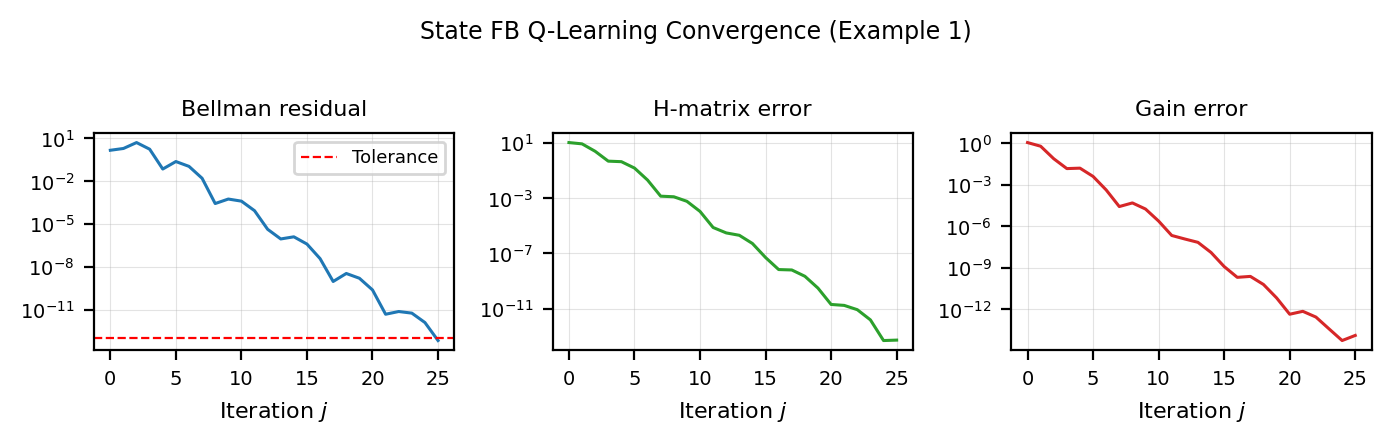
\includegraphics[width=0.72\textwidth]{fig_ex1_sf_conv.png}\\[2pt]
    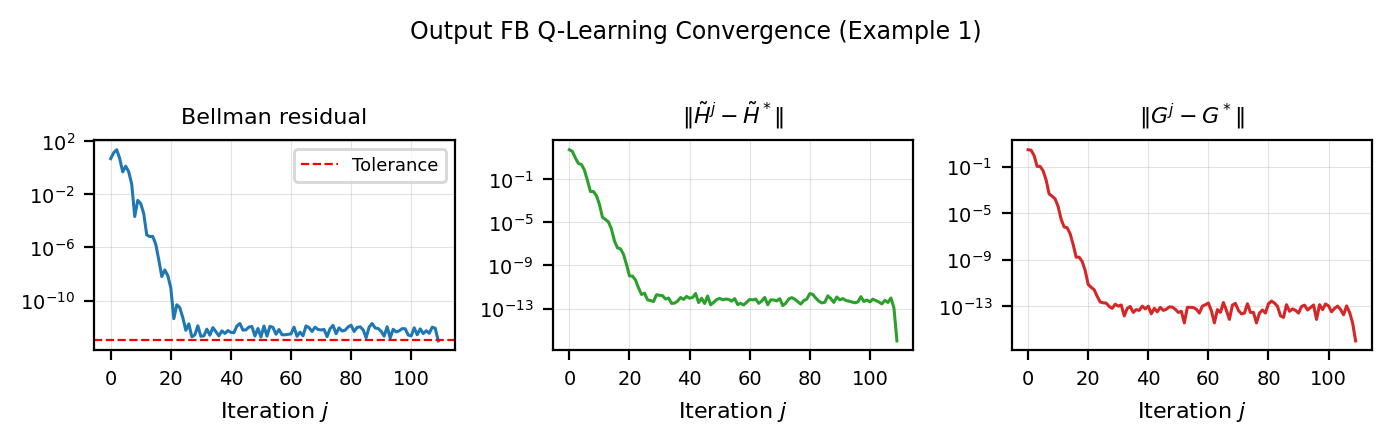
\includegraphics[width=0.72\textwidth]{fig_ex1_of_conv.png}
    \caption{Q-learning convergence for Example~1. Top row: state feedback (Bellman residual, H-matrix error, gain error). Bottom row: output feedback.}
    \label{fig:conv_ex1}
\end{figure*}
Fig.~\ref{fig:traj_ex1} (right) shows the multi-consensus trajectories under the output-feedback deployment~\eqref{eq:ofb_deploy}, with the disagreement reconstructed from the filter states. The trajectories coincide with the state feedback case to within $1.9 \times 10^{-12}$ (Fig.~\ref{fig:of_prop1}, right), which is the quantitative content of Proposition~\ref{prop:disagreement}: output feedback loses nothing.
\begin{figure*}[!t]
    \centering
    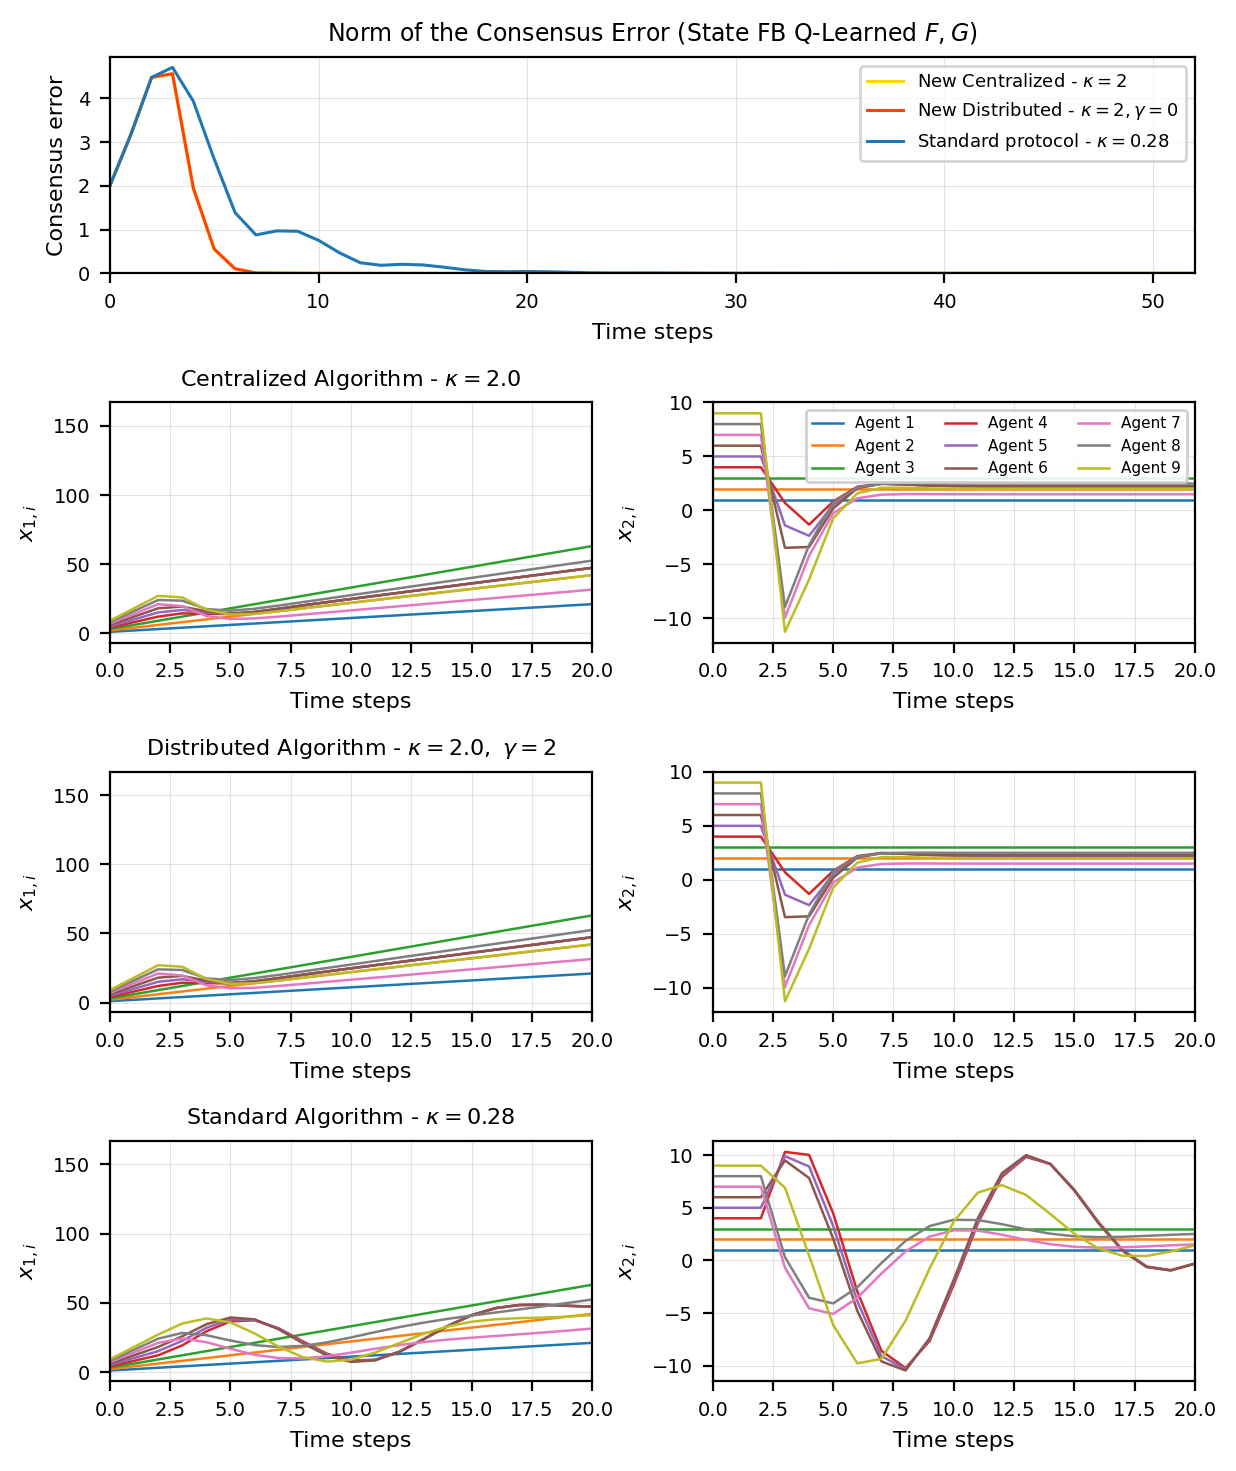
\includegraphics[width=0.42\textwidth]{fig_ex1_sf_traj.png}\hfil
    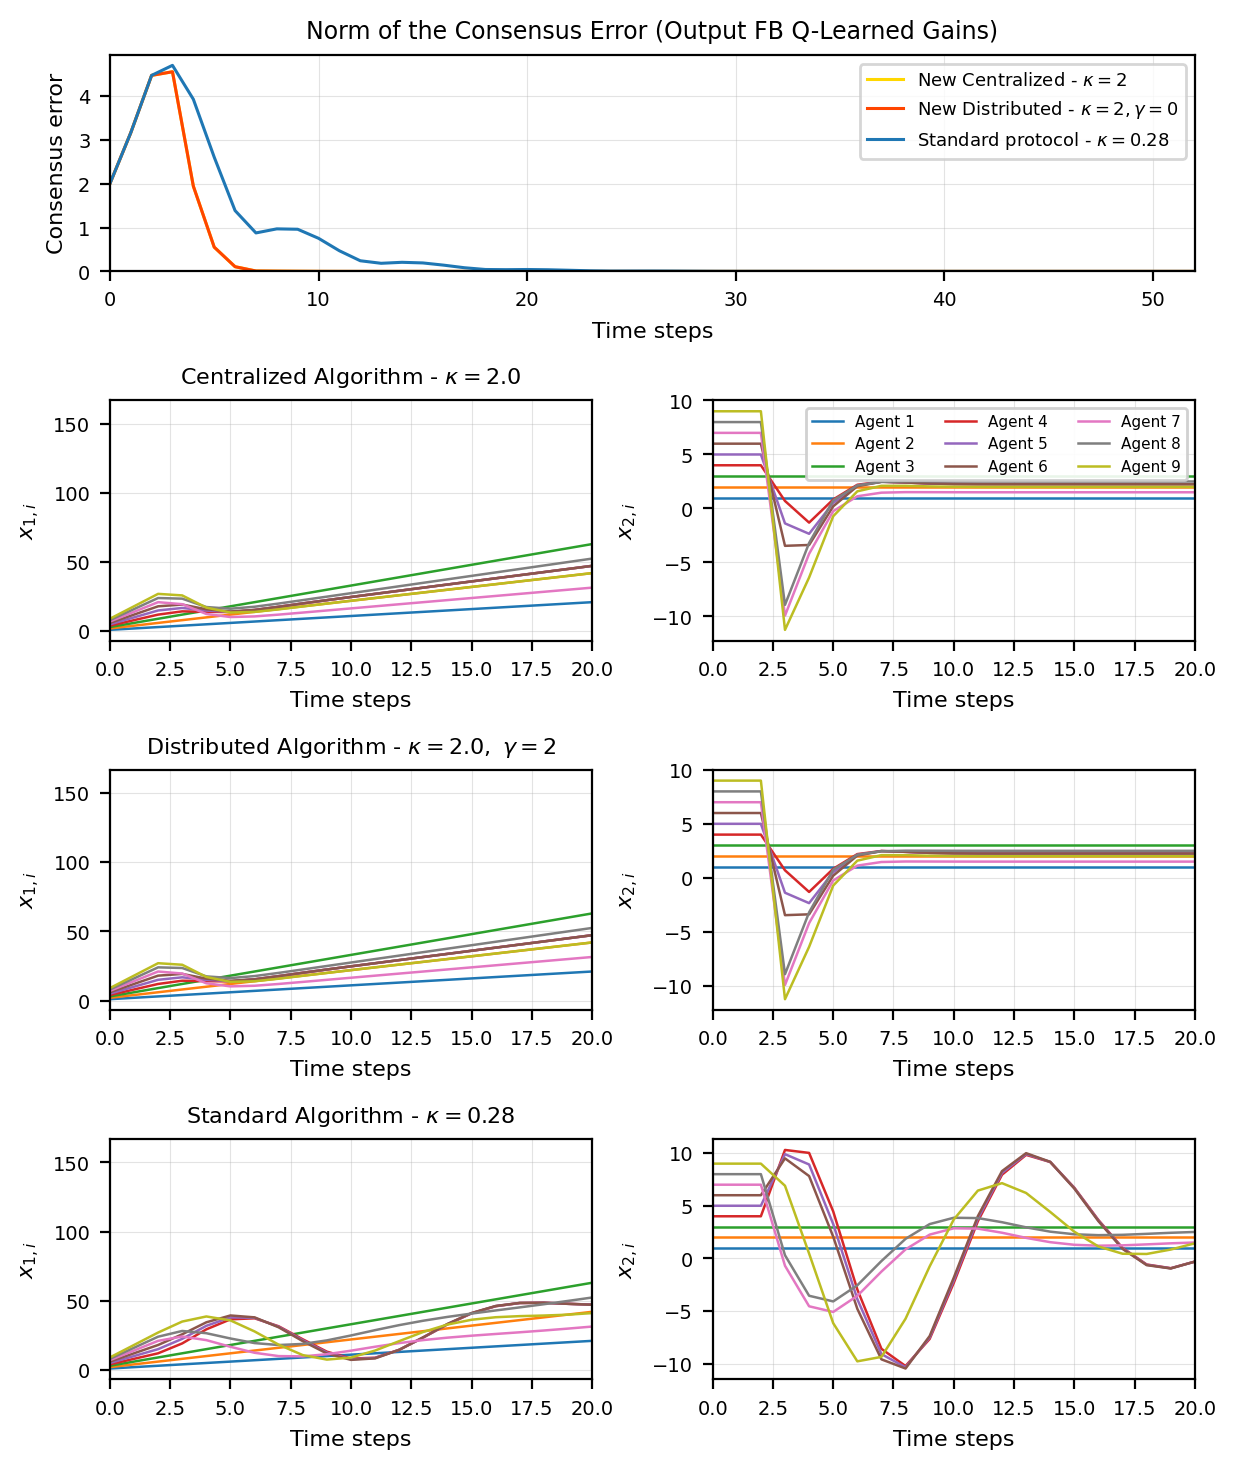
\includegraphics[width=0.42\textwidth]{fig_ex1_of_traj.png}
    \caption{Multi-consensus trajectories for Example~1. Left: state feedback Q-learned gains (top: consensus error; rows 2--4: centralized, distributed with $\gamma = 2$, standard protocol; the first $n = 2$ steps are the zero-input warm-up). Right: output feedback deployment via the reconstructed disagreement~\eqref{eq:disagreement}; the two coincide to machine precision, validating Proposition~\ref{prop:disagreement}.}
    \label{fig:traj_ex1}
\end{figure*}
\subsection{Example 2: Formation Control ($N = 6$, $T = 0.1$~s)}
\label{subsec:sim2}
We consider $N = 6$ continuous-time double integrator agents over the ring digraph in Fig.~\ref{fig:graph6}, which has one reach. Setting $x_i = \col(\zeta_i - \sigma_i, \dot{\zeta}_i)$, the discrete-time model with $T = 0.1$~s has $n = 4$ states and $m = 2$ inputs, and position-only measurements $C = [\,I_2 \;\; 0\,]$ ($p = 2$). We use $Q_y = 5I_2$, hence $Q = C^\top Q_y C$ (Lemma~\ref{lem:psdQ}), for both feedback types so that the state and output feedback designs solve the same LQR problem. The nonzero Laplacian eigenvalues of the directed ring satisfy $\bar{r} = 1 - \cos(2\pi/6) = 0.5$ \emph{exactly}, so the coupling gain must satisfy $\kappa > 2$ strictly; we take $\kappa = 2.5$, giving $\kappa\bar{r} = 1.25 > 1$. The formation is a regular hexagon, representative of UAV coordination problems~\cite{dony2021distributed,dony2021robust}; the data-driven approach is relevant here because the discrete-time model $A = \exp(A_c T)$ inherits unavoidable discretization error.
\begin{figure}[!htbp]
\centering
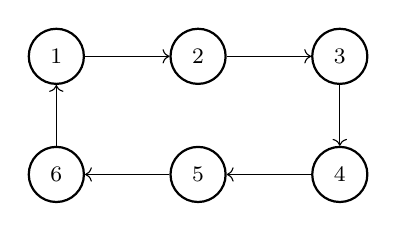
\begin{tikzpicture}[
    node distance=1.8cm,
    every node/.style={circle, draw, minimum size=0.7cm, font=\footnotesize, thick},
    every edge/.style={draw, -Stealth, thick}
]
\node (1) at (0, 1.5) {1};
\node (2) at (1.8, 1.5) {2};
\node (3) at (3.6, 1.5) {3};
\node (6) at (0, 0) {6};
\node (5) at (1.8, 0) {5};
\node (4) at (3.6, 0) {4};
\draw[->] (1) -- (2);
\draw[->] (2) -- (3);
\draw[->] (3) -- (4);
\draw[->] (4) -- (5);
\draw[->] (5) -- (6);
\draw[->] (6) -- (1);
\end{tikzpicture}
\caption{Ring digraph for Example~2 ($N=6$, $\mu=1$, $\bar{r}=0.5$).}
\label{fig:graph6}
\end{figure}
The model-based gains are
\begin{equation*}
F = \begin{bmatrix} 2.4853 & 0 & 2.4780 & 0 \\ 0 & 2.4853 & 0 & 2.4780 \end{bmatrix}, \qquad
G = 0.2354\, I_2 .
\end{equation*}
\subsubsection{State Feedback Results}
With $l = 6$, $N_p = 21$, Fig.~\ref{fig:conv_ex2} (top row) shows convergence in 156 iterations with $\|F - F^*\| < 10^{-12}$. Fig.~\ref{fig:sf_traj_ex2} shows the agents converging to the hexagonal formation within ${\sim}5$~s under both the centralized protocol and its distributed $\gamma$-step approximation with $\gamma = 35$, selected empirically so that the distributed input matches the centralized input to below $10^{-14}$ (Section~\ref{subsec:gamma}).


\subsubsection{Output Feedback Results}
With $\tilde{l} = mn + pn + m = 18$ and $\tilde{N}_p = 171$, output feedback Q-learning converges in 137 iterations with $\|G - G^*\| < 10^{-12}$ (Fig.~\ref{fig:conv_ex2}, bottom row). Fig.~\ref{fig:ofb_traj_ex2} shows the formation trajectories deployed via the reconstructed disagreement~\eqref{eq:disagreement} using position measurements only: the trajectories coincide with the state feedback case to within $8.8 \times 10^{-13}$ (Fig.~\ref{fig:of_prop1}, right).
\begin{figure*}[!t]
    \centering
    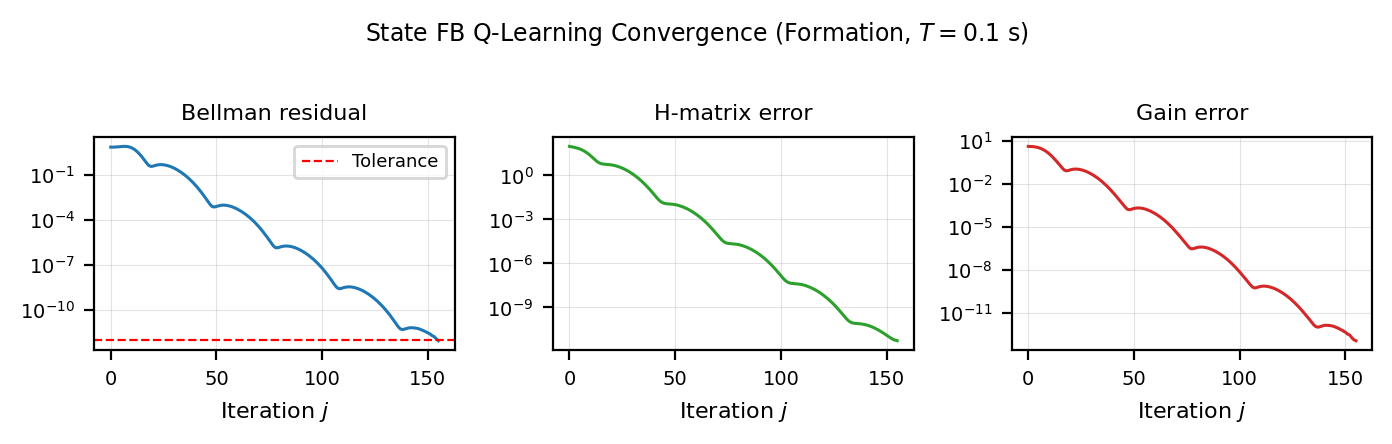
\includegraphics[width=0.72\textwidth]{fig_form_sf_conv.png}\\[2pt]
    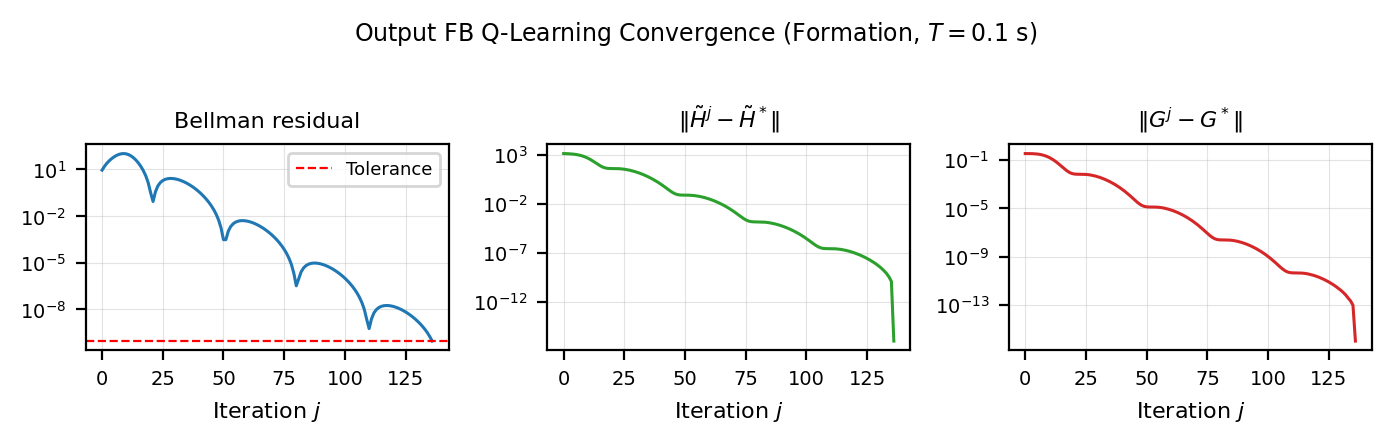
\includegraphics[width=0.72\textwidth]{fig_form_of_conv.png}
    \caption{Q-learning convergence for Example~2 ($T = 0.1$~s). Top row: state feedback. Bottom row: output feedback.}
    \label{fig:conv_ex2}
\end{figure*}
\begin{figure}[!htb]
    \centering
    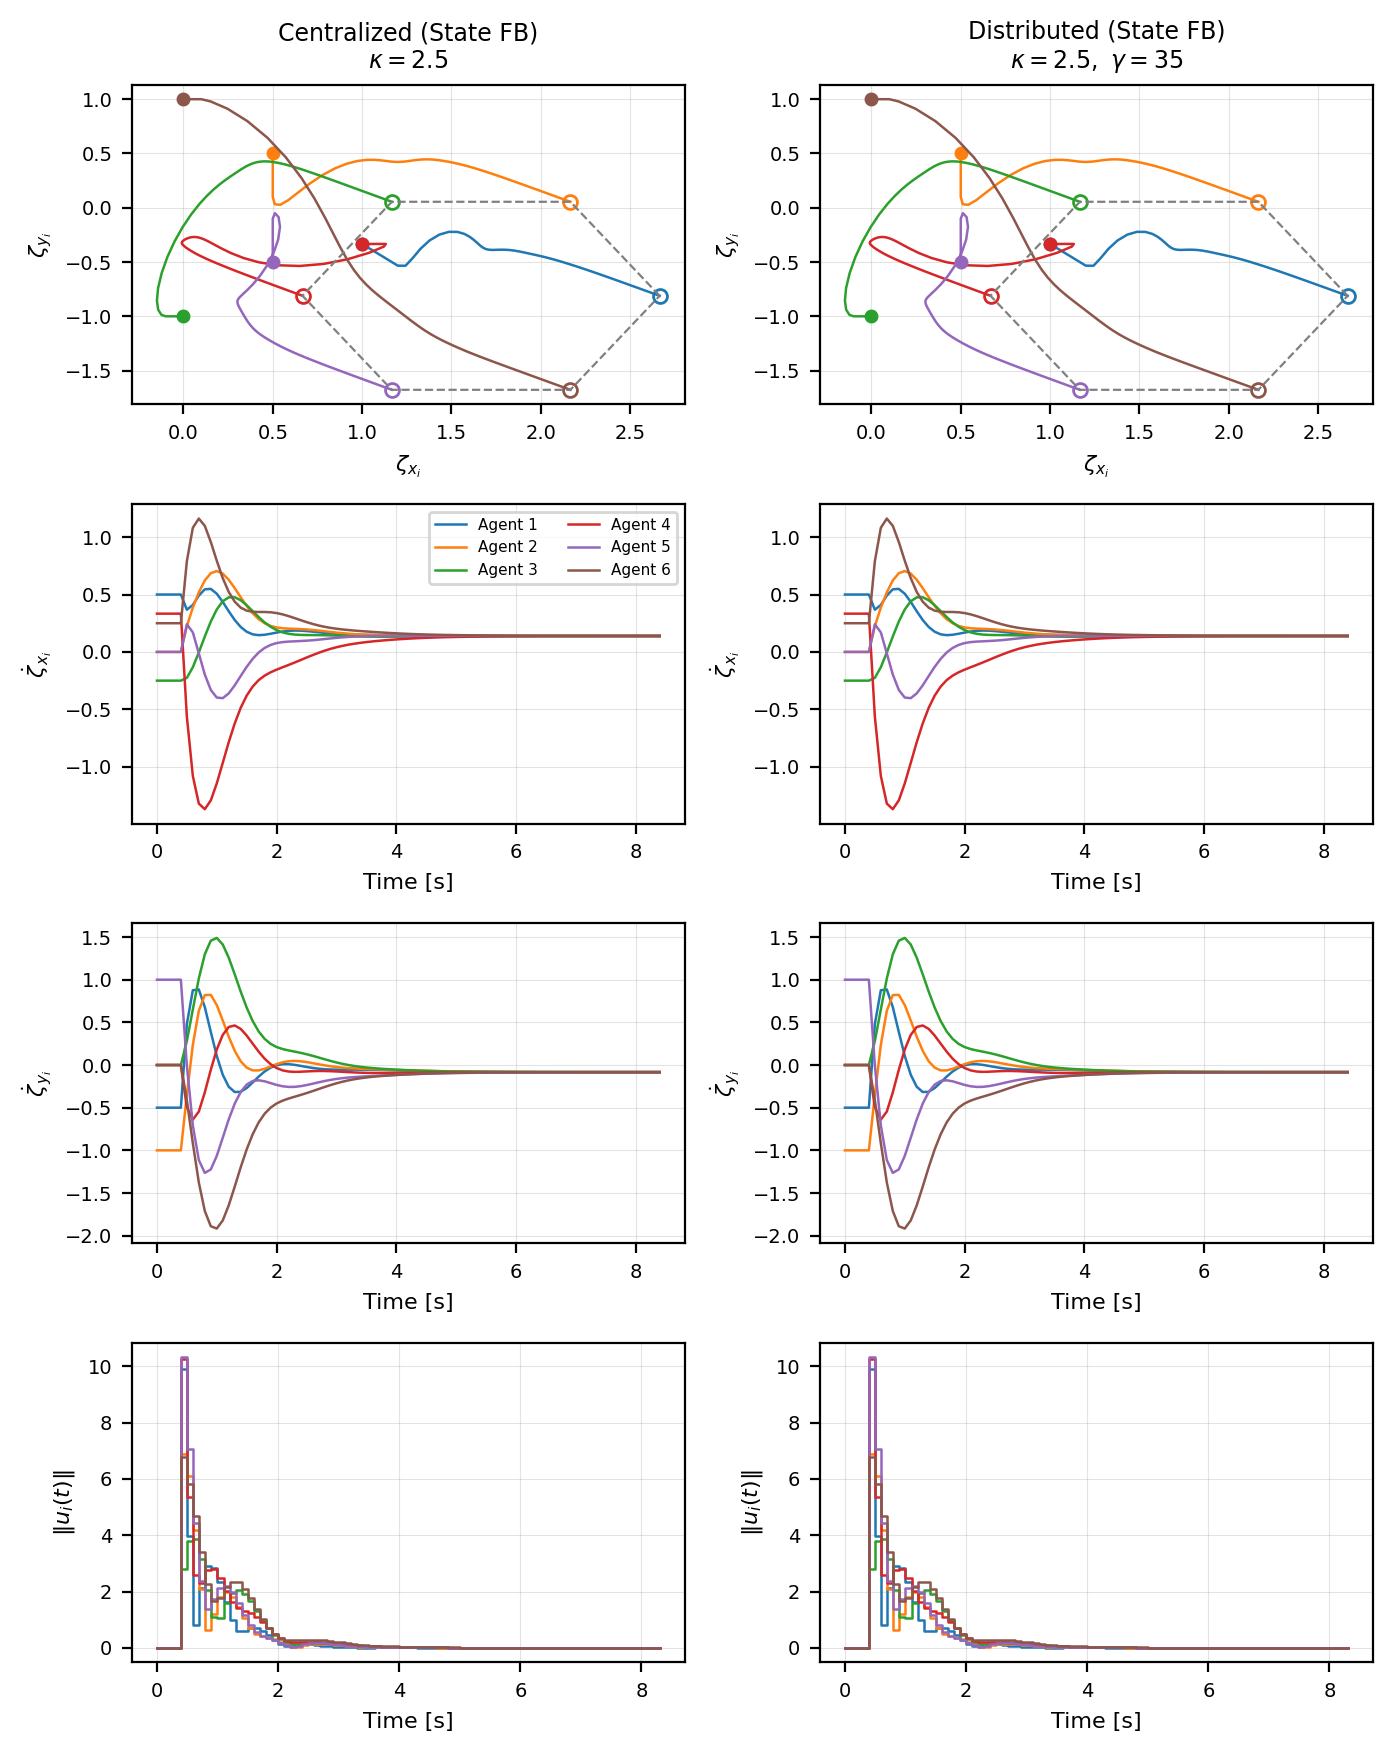
\includegraphics[width=\columnwidth]{fig_form_sf_traj.png}
    \caption{Formation control for Example~2 with state feedback Q-learned gains ($T = 0.1$~s, $\kappa = 2.5$). Left column: centralized; right column: distributed ($\gamma = 35$). Agents converge to the hexagonal formation within ${\sim}5$~s.}
    \label{fig:sf_traj_ex2}
\end{figure}
\begin{figure*}[!t]
    \centering
    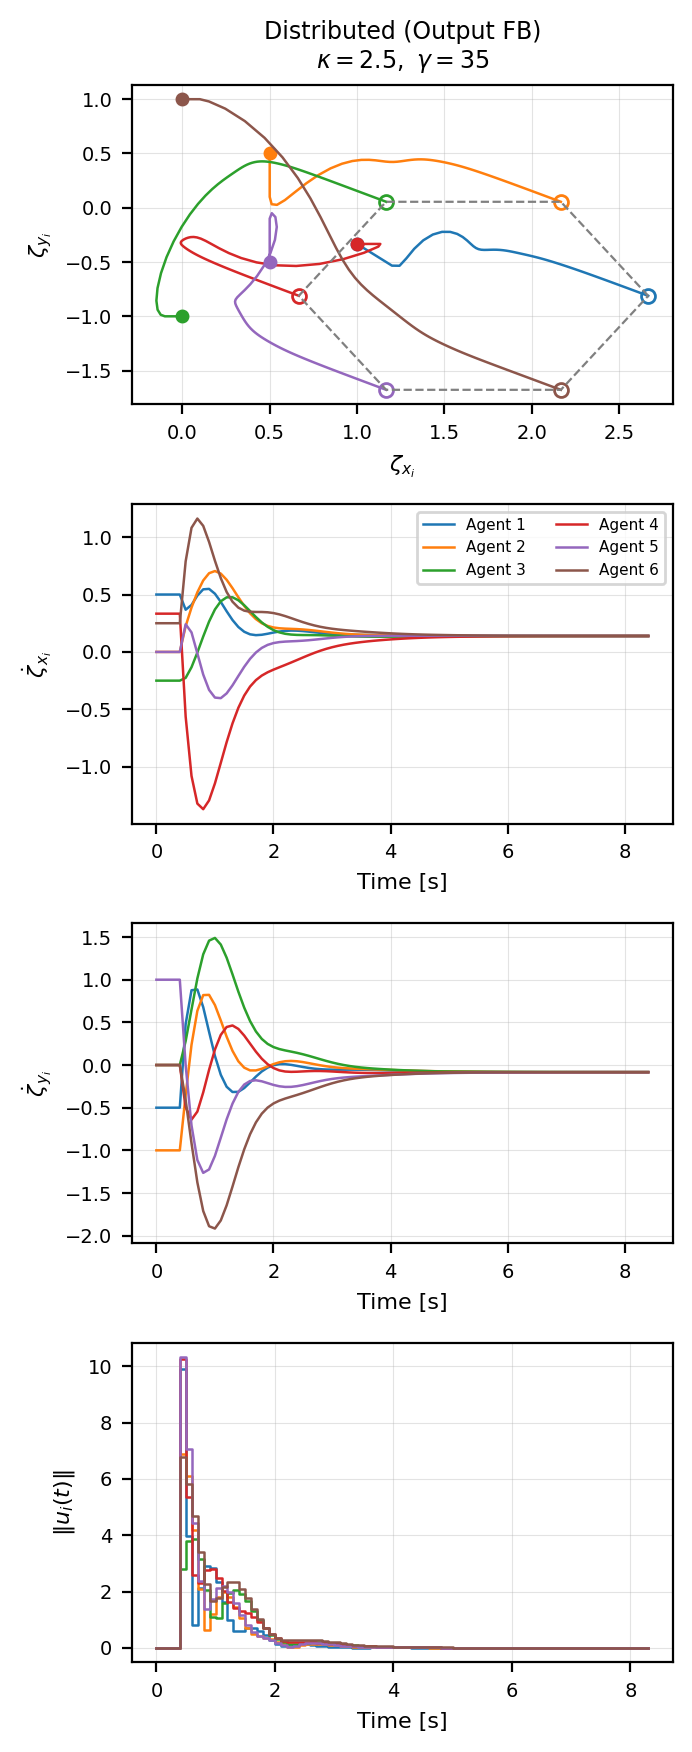
\includegraphics[width=0.3\textwidth]{fig_form_of_traj.png}
    \caption{Formation control for Example~2 with output feedback Q-learned gains, position measurements only ($C = [I_2\;0]$), deployed via the reconstructed disagreement~\eqref{eq:disagreement}. The trajectories coincide with Fig.~\ref{fig:sf_traj_ex2} to machine precision.}
    \label{fig:ofb_traj_ex2}
\end{figure*}
\subsection{Robustness to Parametric Uncertainty}
\label{subsec:robustness}
Because the Bellman equations~\eqref{eq:bellman_consensus} and~\eqref{eq:ofb_bellman} are built entirely from measured data, the Q-learned gains are matched to the true plant from which the data is collected. To quantify this advantage under model uncertainty, we consider Example~1 with a perturbed system matrix $A_{\mathrm{true}} = A_{\mathrm{nom}} + \Delta A$, where $\Delta A = \delta \begin{bsmallmatrix} 0 & 1 \\ 0 & 0 \end{bsmallmatrix}$ represents uncertainty in the $(1,2)$ entry of the double integrator. The model-based approach computes gains from the nominal $A_{\mathrm{nom}}$ via the DARE, while Q-learning extracts gains from data collected on the true (perturbed) system. Since the state and output feedback algorithms recover the identical $(F,G)$ (Theorems~\ref{thm:sf_convergence} and~\ref{thm:ofb_convergence}), a single Q-learned series represents both.

Fig.~\ref{fig:robustness} presents four analyses. Panel~(a) shows that, in this example, the maximum closed-loop spectral radius $\max_k \rho(\bar{A}_k)$ for the model-based gains increases monotonically with the perturbation magnitude, approaching the stability boundary $\rho = 1$, while the Q-learned spectral radius \emph{decreases} over the tested range. At $\delta = 1.0$, the model-based margin is $1 - 0.832 = 0.168$ versus $1 - 0.196 = 0.804$ for Q-learning---a $4.8\times$ improvement. Panel~(b) shows that the relative LQR cost penalty of model-based gains grows to $114\%$ at $\delta = 1.0$ ($J_{\mathrm{nom}}/J_{\mathrm{QL}} = 2.14$). Panel~(c) shows the velocity trajectories at $\delta = 0.3$: the Q-learned gains (dashed) achieve tighter consensus than the model-based gains (solid), consistent with the spectral radius difference. Panel~(d) compares the gain values at $\delta = 0.5$: the Q-learned gains $(2.338,\, 6.803,\, 4.465)$ match the true DARE solution to machine precision, while the nominal model gains $(2,\, 4,\, 3)$ deviate significantly.
\begin{figure*}[!t]
    \centering
    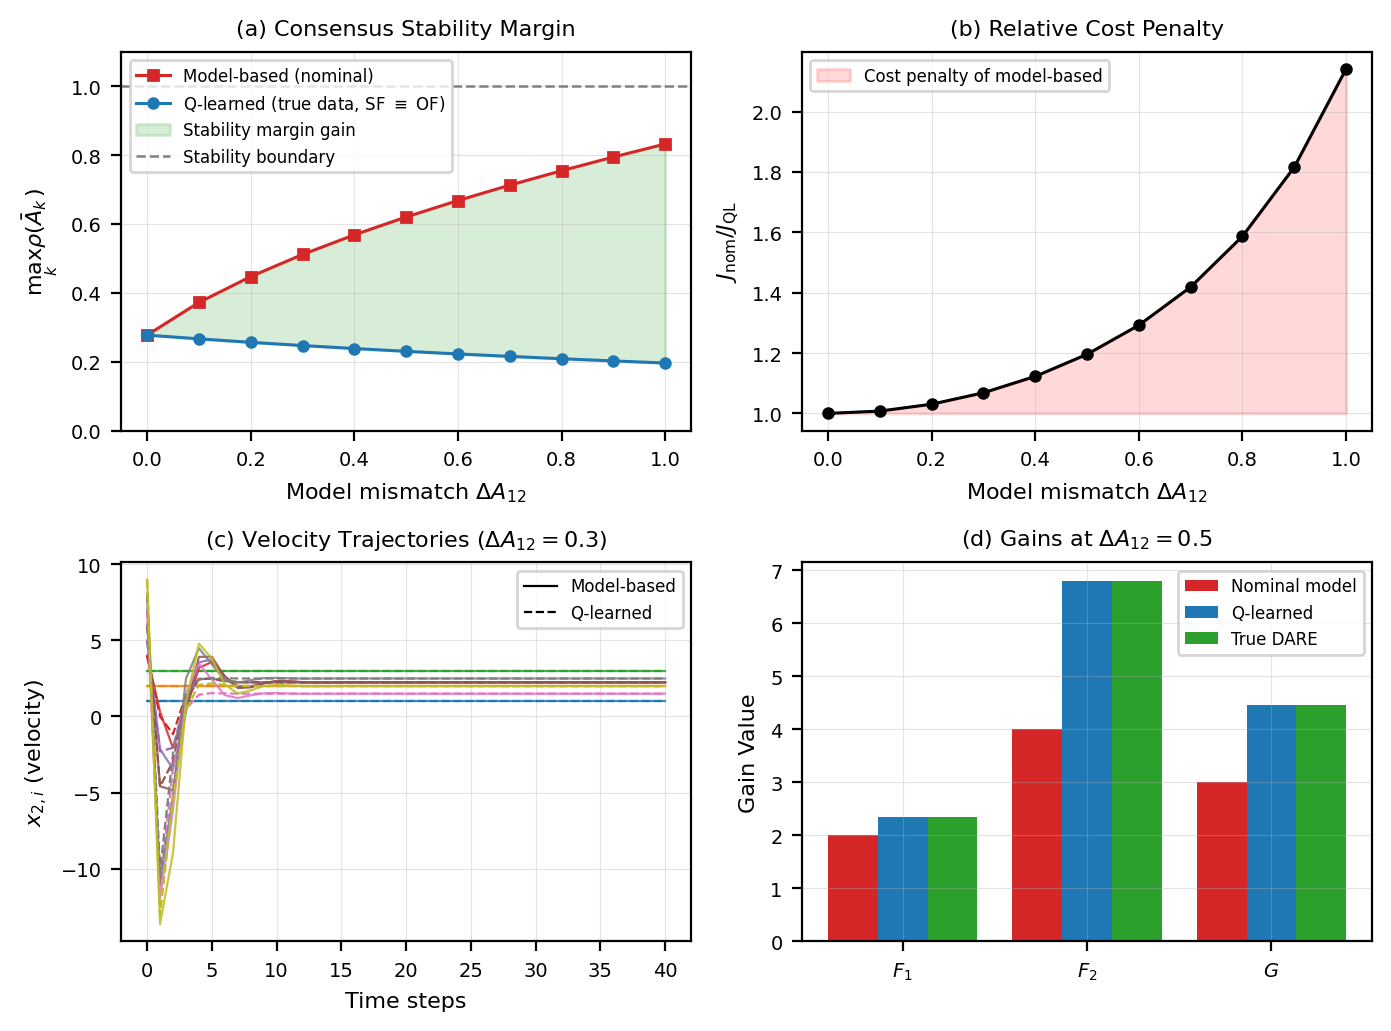
\includegraphics[width=0.75\textwidth]{fig_robustness.png}
    \caption{Robustness analysis under parametric uncertainty $\Delta A_{12}$. Top-left: stability margin (the Q-learned series represents both state and output feedback, which learn identical gains). Top-right: cost penalty. Bottom-left: velocity trajectories at $\delta = 0.3$ (solid = model-based, dashed = Q-learned). Bottom-right: gain comparison at $\delta = 0.5$.}
    \label{fig:robustness}
\end{figure*}
\subsection{Example 3: Vehicle Platoon with Aerodynamic Drag}
\label{subsec:sim4}
A string of $N = 5$ vehicles with aerodynamic drag must achieve velocity consensus while maintaining a desired inter-vehicle spacing of $d_{\mathrm{ref}} = 10$~m. Each vehicle has the discrete-time dynamics
\begin{equation}
A = \begin{bmatrix} 1 & T \\ 0 & 1 - bT \end{bmatrix}, \quad B = \begin{bmatrix} T^2/2 \\ T \end{bmatrix},
\label{eq:platoon}
\end{equation}
where $T = 0.1$~s is the sampling period and $b = 0.1$~s$^{-1}$ is the drag coefficient, adding velocity-dependent dissipation absent from the double integrator. The state is $x_i = [\zeta_i + d_{\mathrm{ref}}\, i, \; \dot{\zeta}_i]^\top$ (spacing coordinate and velocity), the measurement is position only, $C = [1 \;\; 0]$ with $Q_y = 1$, and the communication graph is a directed string $1 \to 2 \to 3 \to 4 \to 5$ with $\bar{r} = 1$ and $\kappa = 2$. The model-based gains are $F = [\,1.0684 \;\; 1.4555\,]$, $G = 0.1416$.

Under state feedback, Algorithm~\ref{alg:sf_ql} converges in 234 iterations with $\|F - F^*\| < 10^{-13}$ (Fig.~\ref{fig:plat_conv}, top row); under output feedback, Algorithm~\ref{alg:ofb_ql} converges in 208 iterations with $\|G - G^*\| < 10^{-12}$ (Fig.~\ref{fig:plat_conv}, bottom row). Fig.~\ref{fig:plat_traj} (top) shows the platoon behavior under the state feedback deployment ($\gamma = 6$): vehicles achieve the desired 10~m spacing with velocity consensus, and control inputs remain smooth and bounded. Fig.~\ref{fig:plat_traj} (bottom) shows the same scenario under the output feedback deployment using position sensors only: the trajectories coincide with the state feedback case to within $8.6 \times 10^{-12}$ (Fig.~\ref{fig:of_prop1}, right), confirming that the platoon can be controlled without velocity measurement.
\begin{figure*}[!t]
    \centering
    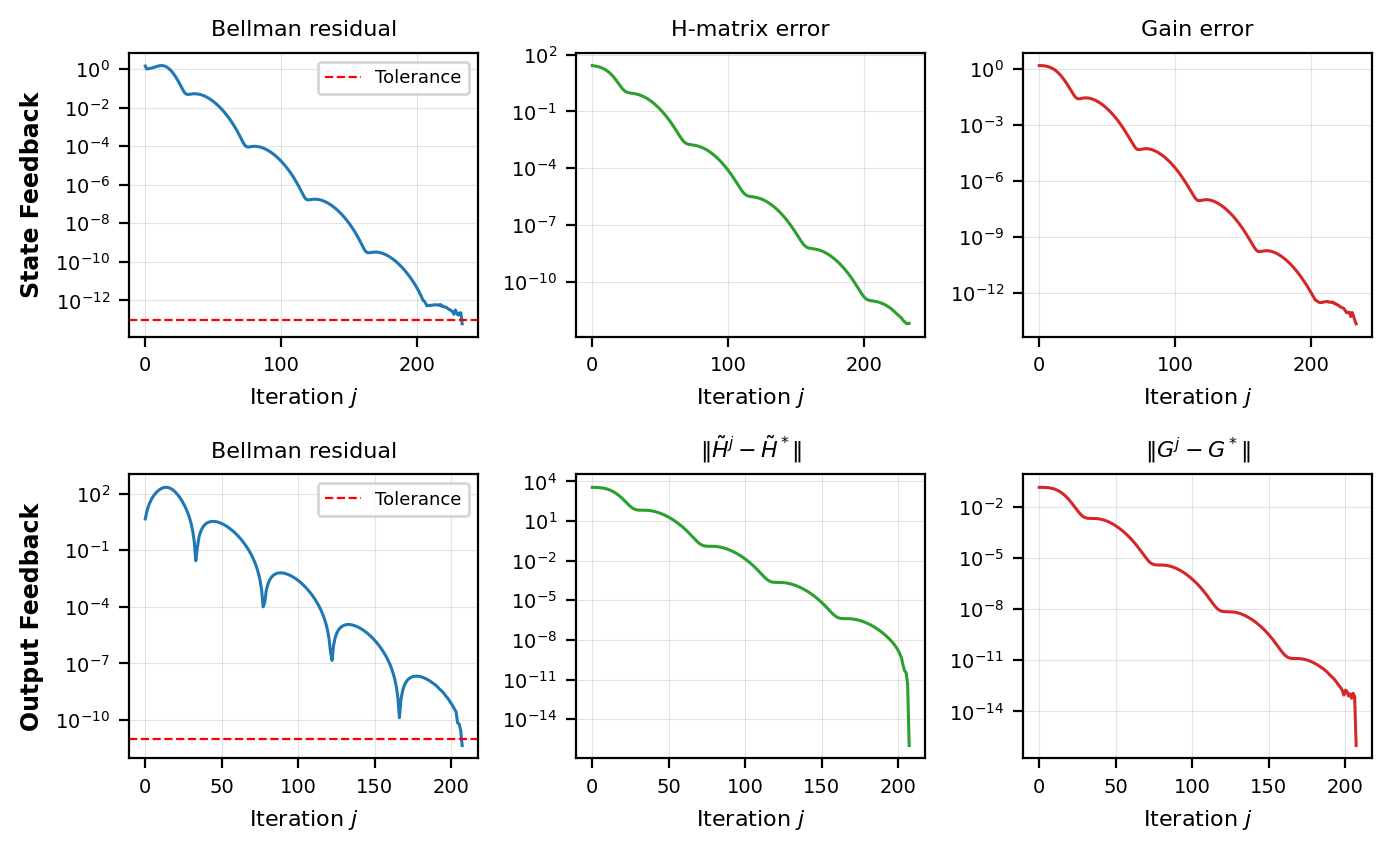
\includegraphics[width=0.72\textwidth]{fig_plat_conv.png}
    \caption{Q-learning convergence for the platoon example. Top row: state feedback. Bottom row: output feedback.}
    \label{fig:plat_conv}
\end{figure*}

\begin{figure*}[!t]
    \centering
    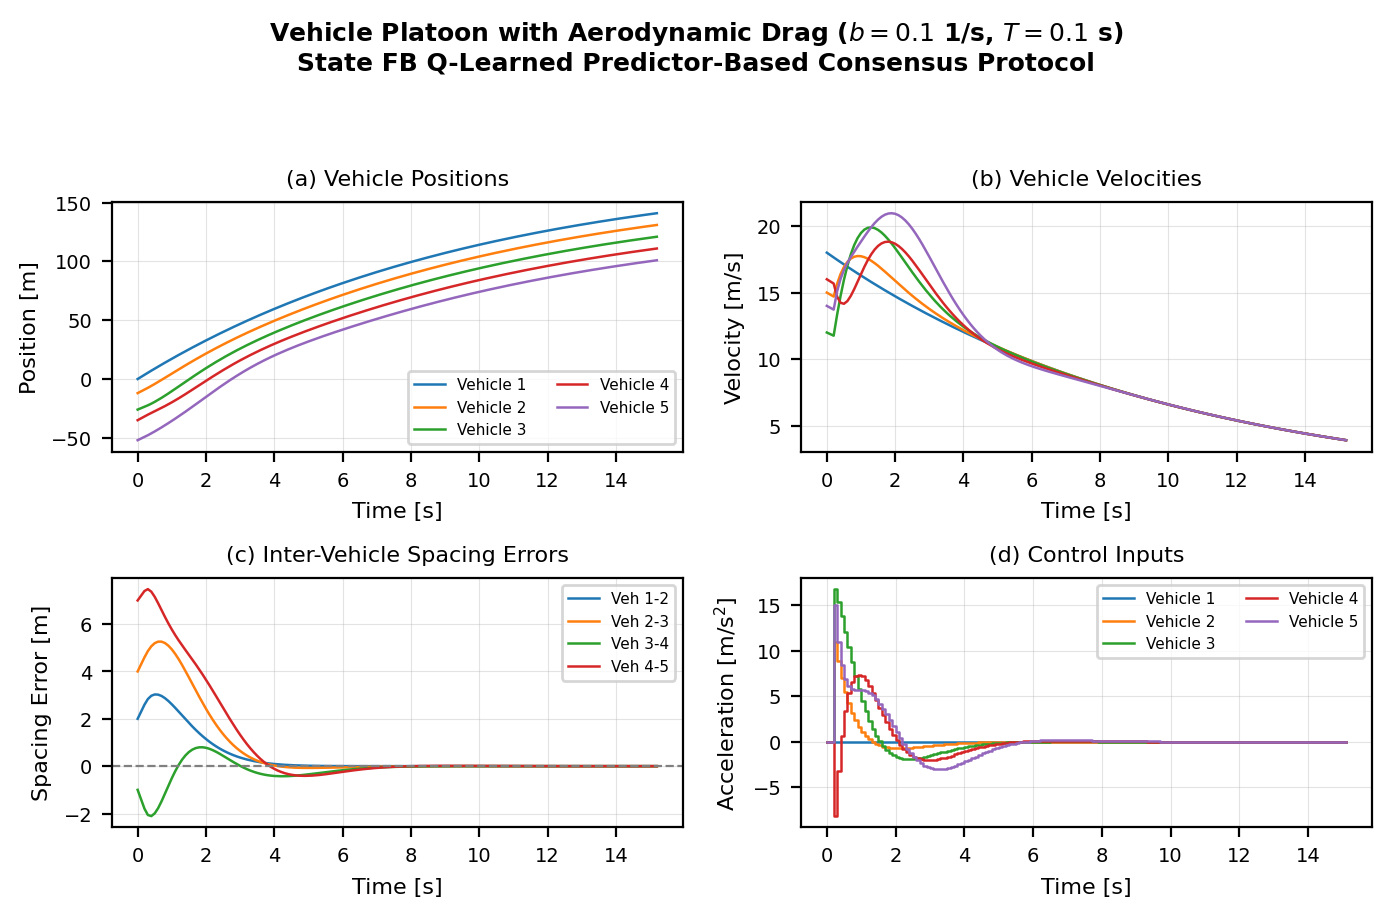
\includegraphics[width=0.66\textwidth]{fig_plat_sf_traj.png}\\[4pt]
    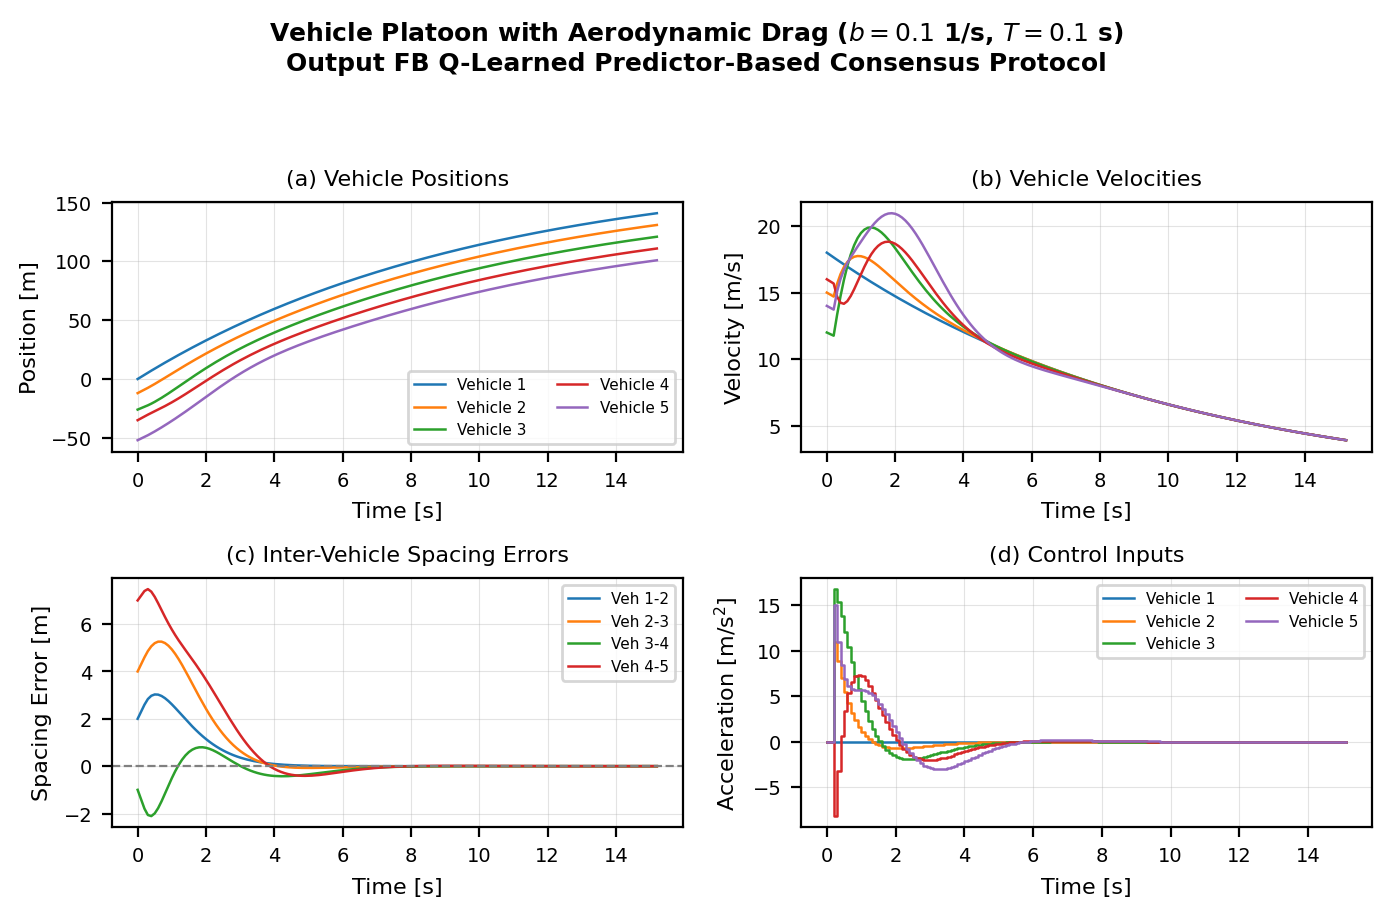
\includegraphics[width=0.66\textwidth]{fig_plat_of_traj.png}
    \caption{Vehicle platoon control ($N=5$, $b=0.1$~s$^{-1}$, $T=0.1$~s). Top: state feedback Q-learned gains ((a) positions, (b) velocities, (c) spacing errors, (d) control inputs). Bottom: output feedback deployment with position sensors only; the trajectories coincide with the state feedback case to machine precision.}
    \label{fig:plat_traj}
\end{figure*}
\subsection{Summary of Results}
\label{subsec:sim_summary}
Table~\ref{tab:summary} summarizes convergence across all examples. Every example is validated under both feedback types, and in every case the output feedback deployment reproduces the state feedback deployment to machine precision.
\begin{table}[htbp]
\centering
\caption{Summary of Q-learning convergence across examples.}
\label{tab:summary}
\small
\setlength{\tabcolsep}{4pt}
\resizebox{\columnwidth}{!}{%
\begin{tabular}{lccccc}
\toprule
Example & $n$ & $m$ & Method & Iterations & Final accuracy \\
\midrule
1 ($N{=}9$, $\mu{=}3$) & 2 & 1 & State FB & 26 & $\|F-F^*\| < 10^{-13}$ \\
& & & Output FB & 110 & $\|G - G^*\| < 10^{-12}$ \\
& & & \multicolumn{2}{r}{OF vs.\ SF deployment} & $< 1.9\times 10^{-12}$ \\
\midrule
2 (Formation, $T{=}0.1$~s) & 4 & 2 & State FB & 156 & $\|F-F^*\| < 10^{-12}$ \\
& & & Output FB & 137 & $\|G - G^*\| < 10^{-12}$ \\
& & & \multicolumn{2}{r}{OF vs.\ SF deployment} & $< 8.8\times 10^{-13}$ \\
\midrule
3 (Platoon) & 2 & 1 & State FB & 234 & $\|F-F^*\| < 10^{-13}$ \\
& & & Output FB & 208 & $\|G - G^*\| < 10^{-12}$ \\
& & & \multicolumn{2}{r}{OF vs.\ SF deployment} & $< 8.6\times 10^{-12}$ \\
\bottomrule
\end{tabular}}
\end{table}
\FloatBarrier
%% ===================================================================
\section{Discussion}
\label{sec:discussion}
%% ===================================================================
This section analyzes the practical properties of the framework: computational cost, scalability, selection of the iteration depth $\gamma$, communication requirements, the nature of the robustness advantage, and limitations.
\subsection{Computational Complexity}
\label{subsec:complexity}
Each iteration of Algorithm~\ref{alg:sf_ql} solves an $l(l+1)/2$-dimensional least-squares problem at cost $\mathcal{O}(N_d \cdot l^2 + l^6)$, for a total of $\mathcal{O}(J \cdot l^6)$ over $J$ iterations, versus $\mathcal{O}(n^3)$ for the model-based DARE via Schur decomposition; the premium buys freedom from system identification and its errors. The output-feedback algorithm is identical with $\tilde{l} = mn+pn+m$ in place of $l$: the larger regression ($\tilde{N}_p = 171$ vs.\ $N_p = 21$ in Example~2) raises per-iteration cost and data length, while iteration counts remain comparable (137 vs.\ 156, Table~\ref{tab:summary}).
\subsection{Scalability with Network Size}
\label{subsec:scalability}
Since the DARE depends only on $(A,B,Q)$ and not on the graph, Algorithms~\ref{alg:sf_ql}--\ref{alg:ofb_ql} run once on a single agent and the gains deploy across all $N$ agents: the learning phase is identical for 5 or 500 agents. This contrasts with distributed RL methods such as~\cite{zhang2011}, where every agent learns concurrently and the cost scales with $N$.
\subsection{Model-Free Selection of the Distributed Iteration Depth $\gamma$}
\label{subsec:gamma}
The minimum number of distributed consensus steps $\gamma_{\min}$ from~\cite[Thm.~3.4]{cacace2024} depends on $\rho(G)$ and $\rho(A - BK^*)$. The spectral radius $\rho(G) = \rho(H_{uu}^* - I_m)$ is directly available from the converged H-matrix without any model knowledge. Quantities involving the closed-loop matrix $A - BK^*$, however, are not directly available from $H^*$ alone. In a fully data-driven implementation, one may collect closed-loop data under the converged policy $K^*$ and estimate
\begin{equation}
\hat{A}_{\mathrm{cl}} = X^+ X^\dagger,
\label{eq:Acl}
\end{equation}
where $X = [x_0, \ldots, x_{T-1}]$, $X^+ = [x_1, \ldots, x_T]$, and $X^\dagger$ denotes the pseudoinverse; then $\rho(A - BK^*)$ is approximated by $\rho(\hat{A}_{\mathrm{cl}})$. Alternatively, $\gamma$ can be selected empirically by increasing the number of inner consensus iterations until the distributed input $v_i(t,\gamma)$ is sufficiently close to the centralized input~\eqref{eq:u_central}, which is the procedure used in Example~2: $\gamma = 20$ already gives a state deviation below $1.2\times10^{-9}$, and $\gamma = 35$ reaches numerical precision ($7\times10^{-15}$).
\subsection{Communication Requirements}
\label{subsec:communication}
The $\gamma$-step algorithm~\eqref{eq:dist_init}--\eqref{eq:dist_iter} costs $\gamma$ communication rounds per period: larger $\gamma$ tracks~\eqref{eq:u_central} more closely but latency constrains $\gamma \leq T/\tau_{\mathrm{comm}}$. This requirement is inherited from~\cite{cacace2024}, not introduced by learning---once learned, the gains impose no additional communication; event-triggered variants are a promising direction.
\subsection{Interpretation of the Robustness Results}
\label{subsec:robust_disc}
The robustness study demonstrates \emph{exactness on the true plant}: Q-learning recovers the DARE solution of the perturbed system to machine precision, while the model-based design stays anchored to the nominal model and its margin erodes. This is data-driven exactness, not a formal robustness margin; the $4.8\times$ margin improvement and $114\%$ cost penalty at $\delta = 1.0$ quantify its practical consequence, and the insight transfers to applications such as the platoon of Section~\ref{subsec:sim4}, where parameters like the drag coefficient drift with operating conditions.
\subsection{Limitations}
\label{subsec:limitations}
Three limitations delineate the scope of the present results. First, the framework assumes identical linear agents; heterogeneous or nonlinear dynamics would break the single-agent learning architecture and the quadratic Q-function structure, respectively. Second, the convergence guarantees assume noise-free state or output \emph{measurements}; exploration noise in the input is provably bias-free (Theorems~\ref{thm:sf_convergence} and~\ref{thm:ofb_convergence}), but measurement noise would require an instrumental-variable or total-least-squares treatment. Third, the excitation (rank) condition on the regression matrix must be verified in practice, which constrains the choice of probing signals during the learning phase.
%% ===================================================================
\section{Conclusions}
\label{sec:conc}
%% ===================================================================
This paper presented data-driven Q-learning algorithms for the gains of a predictor-based consensus protocol for discrete-time linear MAS. Exploiting the DARE--LQR equivalence, the state feedback algorithm extracts both gains from single-agent data; the output feedback extension, building on~\cite{rizvi2022}, reconstructs the inter-agent disagreement feedback rather than the absolute regulator. The learned gains satisfy the DARE exactly, so all guarantees of~\cite{cacace2024}---including arbitrary convergence rate and multi-consensus---are inherited, with the stability condition extended to the positive semi-definite weights that output feedback necessitates. Every scenario was validated under both feedback types, with the two deployments coinciding to machine precision against the model-based benchmark; the robustness study showed superior margins under parametric uncertainty, and the platoon example confirmed practicality with position-only sensing.
Future directions include heterogeneous MAS (requiring distributed Q-learning), time-varying topologies with event-triggered communication, nonlinear extensions via Koopman lifting~\cite{dony2024koopman}, and safety enforcement through control barrier functions~\cite{dony2025debf}.
%% ===================================================================
\section*{Declaration of Competing Interest}
%% ===================================================================
The authors declare that they have no known competing financial interests or personal relationships that could have appeared to influence the work reported in this paper.
%% ===================================================================
\section*{Funding}
%% ===================================================================
This research did not receive any specific grant from funding agencies in the public, commercial, or not-for-profit sectors.
%% ===================================================================
\section*{Data Availability}
%% ===================================================================
The simulation scripts that support the findings of this study are available from the corresponding author upon reasonable request.
%% ===================================================================
\section*{CRediT Authorship Contribution Statement}
%% ===================================================================
\textbf{Md Nur-A-Adam Dony:} Conceptualization, Methodology, Software, Formal analysis, Investigation, Validation, Writing -- original draft, Visualization.
\textbf{Syed Ali Asad Rizvi:} Conceptualization, Methodology, Supervision, Writing -- review \& editing.
%% ===================================================================
%% References (numbered in order of first appearance)
%% ===================================================================
\begingroup\small
\begin{thebibliography}{99}
\bibitem{francis2016}
B.A. Francis, M. Maggiore, Flocking and Rendezvous in Distributed Robotics, Springer, 2016.
\bibitem{dony2021distributed}
M.N.A. Dony, W. Dong, Distributed robust formation flying and attitude synchronization of spacecraft, J. Aerosp. Eng. 34 (2021) 04021002.
\bibitem{dong2020tracking}
W. Dong, M.N.A. Dony, M. Rafat, Tracking control of vertical taking-off and landing vehicles with parametric uncertainty, Int. J. Adapt. Control Signal Process. 34 (2020) 1600--1612.
\bibitem{dorfler2014}
F. D\"{o}rfler, F. Bullo, Synchronization in complex networks of phase oscillators: A survey, Automatica 50 (6) (2014) 1539--1564.
\bibitem{li2010}
Z. Li, Z. Duan, G. Chen, L. Huang, Consensus of multiagent systems and synchronization of complex networks: A unified viewpoint, IEEE Trans. Circuits Syst. I Reg. Papers 57 (1) (2010) 213--224.
\bibitem{battistelli2014}
G. Battistelli, L. Chisci, G. Mugnai, A. Farina, A. Graziano, Consensus-based linear and nonlinear filtering, IEEE Trans. Autom. Control 60 (5) (2015) 1410--1415.
\bibitem{proskurnikov2017}
A.V. Proskurnikov, R. Tempo, A tutorial on modeling and analysis of dynamic social networks. Part I, Annu. Rev. Control 43 (2017) 65--79.
\bibitem{li2014}
Z. Li, G. Wen, Z. Duan, W. Ren, Designing fully distributed consensus protocols for linear multi-agent systems with directed graphs, IEEE Trans. Autom. Control 60 (4) (2015) 1152--1157.
\bibitem{liu2021}
Z. Liu, A. Saberi, A.A. Stoorvogel, D. Nojavanzadeh, Scale-free collaborative protocol design for state and regulated state synchronization of multi-agent systems with arbitrary fast convergence, J. Franklin Inst. 358 (9) (2021) 4864--4882.
\bibitem{ma2015}
Q. Ma, F.L. Lewis, S. Xu, Cooperative containment of discrete-time linear multi-agent systems, Int. J. Robust Nonlinear Control 25 (7) (2015) 1007--1018.
\bibitem{ren2010}
W. Ren, Y. Cao, Distributed Coordination of Multi-Agent Networks, Springer, 2010.
\bibitem{xiao2004}
L. Xiao, S. Boyd, Fast linear iterations for distributed averaging, Syst. Control Lett. 53 (1) (2004) 65--78.
\bibitem{cacace2024}
F. Cacace, M. Mattioni, S. Monaco, D. Normand-Cyrot, Consensus and multi-consensus for discrete-time LTI systems, Automatica 166 (2024) 111718.
\bibitem{monaco2019}
S. Monaco, L. Ricciardi~Celsi, On multi-consensus and almost equitable graph partitions, Automatica 103 (2019) 53--61.
\bibitem{dony2020tracking}
M.N.A. Dony, M. Rafat, W. Dong, Distributed command filtered robust tracking control of wave-adaptive modular vessel with uncertainty, in: Proc. 2020 American Control Conference (ACC), Denver, CO, 2020, pp. 2118--2123.
\bibitem{dony2021robust}
M.N.A. Dony, Robust Distributed Formation Control of UAVs with Higher-Order Dynamics, Master's thesis, The University of Texas Rio Grande Valley, 2021.
\bibitem{lewis2009}
F.L. Lewis, D. Vrabie, Reinforcement learning and adaptive dynamic programming for feedback control, IEEE Circuits Syst. Mag. 9 (3) (2009) 32--50.
\bibitem{bradtke1994}
S.J. Bradtke, B.E. Ydstie, A.G. Barto, Adaptive linear quadratic control using policy iteration, in: Proc. American Control Conference, 1994, pp. 3475--3479.
\bibitem{rizvi2022}
S.A.A. Rizvi, Z. Lin, Output Feedback Reinforcement Learning Control for Linear Systems, Control Engineering Series, Springer Nature, 2022.
\bibitem{zhang2011}
H. Zhang, F.L. Lewis, A. Das, Optimal design for synchronization of cooperative systems: State feedback, observer and output feedback, IEEE Trans. Autom. Control 56 (8) (2011) 1948--1952.
\bibitem{dony2025debf}
M.N.A. Dony, M.E. Khallil, Adaptive reinforcement learning with control barrier functions for safe state avoidance in discrete event systems, in: Proc. 8th IEOM Bangladesh Int. Conf., Dhaka, Bangladesh, 2025.
\bibitem{dony2026battery}
M.N.A. Dony, B. Arhin, Data-driven distributed battery state-of-charge balancing using neural network-based open circuit voltage learning, IFAC J. Syst. Control 36 (2026) 100415.
\bibitem{dony2024koopman}
M.N.A. Dony, Integrating Koopman theory and Lyapunov stability for enhanced model predictive control in nonlinear systems, ResearchGate preprint, 2024. https://doi.org/10.13140/RG.2.2.17950.31046.
\bibitem{caughman2006}
J.S. Caughman, J.J.P. Veerman, Kernels of directed graph Laplacians, Electron. J. Combin. 13 (1) (2006) 39.
\bibitem{hewer1971}
G.A. Hewer, An iterative technique for the computation of the steady state gains for the discrete optimal regulator, IEEE Trans. Autom. Control 16 (4) (1971) 382--384.
\end{thebibliography}
\endgroup
\end{document}
